\documentclass[letterpaper,12pt]{article}

\usepackage{algorithm}
\usepackage[noend]{algpseudocode}
\usepackage[table,xcdraw]{xcolor}
\renewcommand{\algorithmicrequire}{\textbf{Input:}}
\renewcommand{\algorithmicensure}{\textbf{Output:}}

% @@@@@@@@@@@@@@@@@@@@@@@@@@@@@@@@@@@@@@@@@@@@@@@@@@@@@@@@@@@@>
% VALORES A MODIFICAR POR USTED:
% @@@@@@@@@@@@@@@@@@@@@@@@@@@@@@@@@@@@@@@@@@@@@@@@@@@@@@@@@@@@>
\usepackage{multirow}
% NOTE: Leer nota en el README sobre la font.

\newcommand{\titulo}{Ishvel: un Framework para la Elaboración de Tareas en Cursos Introductorios de Programación}
\newcommand{\ciudad}{Santiago} % e.g. Valparaíso
% TODO: Consultar el formato de los nombres:
\newcommand{\nombrealumno}{Gonzalo Andrés Fernández Carrillo}
\newcommand{\nombreprofesor}{Federico Meza}
\newcommand{\nombrecorreferente}{Andrea Vásquez}
% Mes y año del examen
\newcommand{\mesexamen}{Agosto}
\newcommand{\anioexamen}{2022}
% Dedicatoria y agradecimientos
\newcommand{\dedicatoria}{

}
\newcommand{\agradecimientos}{

}
\newcommand{\resumen}{

}
\newcommand{\resumeningles}{

}
\newcommand{\palabrasclave}{
Elaborar tareas, framework, curso introductorio de programación, educación
}
\newcommand{\palabrasclaveingles}{
Create assignments, framework, introductory programming course, education
}
% @@@@@@@@@@@@@@@@@@@@@@@@@@@@@@@@@@@@@@@@@@@@@@@@@@@@@@@@@@@@>

% Paquete para importar imágenes
\usepackage{graphicx}
% Directorio de las imágenes
\graphicspath{ {figures/} }

% Idioma y fuentes
\usepackage[spanish,es-tabla]{babel}
\usepackage[T1]{fontenc}

\usepackage{fontspec}
\usepackage[sfdefault,lf]{carlito}



% Tamaño de la página y márgenes
\usepackage[letterpaper,top=2.5cm,bottom=3cm,left=3cm,right=3cm,marginparwidth=1.75cm]{geometry}

% Determinar interlineado:
\renewcommand{\baselinestretch}{1.0}

% Eliminar sangrías:
\setlength{\parindent}{0cm}

% Paquete para definir los formatos de los títulos
\usepackage[explicit]{titlesec}

\titleformat{name=\section}[block]{\fontsize{16}{24}\selectfont\bfseries}{}{0pt}{#1}
\titleformat{name=\section,numberless}[block]{\fontsize{16}{24}\selectfont\bfseries}{}{0pt}{#1}
\titlespacing*{name=\section}{0pt}{0pt}{0.5cm}
\titlespacing*{name=\section,numberless}{0pt}{0pt}{0.5cm}

% Separación entre parrafos
\setlength{\parskip}{0.4cm}

% Paquetes de utilidad general
\usepackage{amsmath}
\usepackage{graphicx}
\usepackage{float}
\usepackage[colorlinks=true, allcolors=blue]{hyperref}

% Formato de las tablas de contenido
% \usepackage[tocflat]{tocstyle}
\usepackage{tocbasic}

% Para obtener el número de la última página
\usepackage{lastpage}

% Header y footer
\usepackage{fancyhdr}
\fancypagestyle{portada}{
    \lhead{}
    \chead{}
    \rhead{}
    \lfoot{}
    \cfoot{\fontsize{10}{12}\selectfont \thepage}
    \rfoot{}
    \renewcommand{\headrulewidth}{0pt}
}
\fancypagestyle{intermedio}{
    \lhead{}
    \chead{\fontsize{10}{12}\selectfont\MakeUppercase{\titulo}}
    \rhead{}
    \lfoot{}
    \cfoot{\fontsize{10}{12}\selectfont Página \textbf{\thepage}\ de \textbf{\pageref{LastPage}}}
    \rfoot{}
    \renewcommand{\headrulewidth}{1pt}
}

% Comandos para secciones
\newcommand{\secnumbersection}[1]{
\addtocounter{section}{1}
\section*{CAPÍTULO \thesection \texorpdfstring{\\}\ #1}
\addcontentsline{toc}{section}{CAPÍTULO \thesection : #1}
\setcounter{subsection}{0}
}
\newcommand{\secnumberlesssection}[1]{
\section*{#1}
\phantomsection
\addcontentsline{toc}{section}{#1}
\setcounter{subsection}{0}
}

% Nombres
\addto\captionsspanish{\renewcommand{\contentsname}{ÍNDICE DE CONTENIDOS}}
\addto\captionsspanish{\renewcommand{\listfigurename}{ÍNDICE DE FIGURAS}}
\addto\captionsspanish{\renewcommand{\listtablename}{ÍNDICE DE TABLAS}}
\makeatletter
\renewenvironment{thebibliography}[1]
     {\secnumberlesssection{REFERENCIAS BIBLIOGRÁFICAS}
      \@mkboth{\MakeUppercase\bibname}{\MakeUppercase\bibname}%
      \list{\@biblabel{\@arabic\c@enumiv}}%
           {\settowidth\labelwidth{\@biblabel{#1}}%
            \leftmargin\labelwidth
            \advance\leftmargin\labelsep
            \@openbib@code
            \usecounter{enumiv}%
            \let\p@enumiv\@empty
            \renewcommand\theenumiv{\@arabic\c@enumiv}}%
      \sloppy
      \clubpenalty4000
      \@clubpenalty \clubpenalty
      \widowpenalty4000%
      \sfcode`\.\@m}
     {\def\@noitemerr
       {\@latex@warning{Empty `thebibliography' environment}}%
      \endlist}
\makeatother

% Personalizar Tabla de Contenidos

\usepackage{tocloft}
\renewcommand{\cftsecfont}{\fontsize{12}{14}\selectfont\fontspec{Carlito}}
\renewcommand{\cftsubsecfont}{\fontsize{12}{14}\selectfont\fontspec{Carlito}}
\renewcommand{\cftsubsubsecfont}{\fontsize{12}{14}\selectfont\fontspec{Carlito}}

\renewcommand\cftfigfont{\fontsize{12}{14}\selectfont\fontspec{Carlito}}

% Links sin color
\usepackage{hyperref}
\hypersetup{colorlinks = false}

% Comando para secciónes sin enumeración
% (sugerido por @anibalbastiass https://github.com/autopawn/tex-thesis-template/issues/5#issuecomment-916106128)
\newcommand{\secnumberlesssubsection}[1]{
\subsection*{#1}
\phantomsection
\addcontentsline{toc}{subsection}{#1}
\setcounter{subsection}{0}
}
% Forma de uso:
% \secnumberlesssubsection{"Sub seccion sin enumeración"}

% @@@@@@@@@@@@@@@@@@@@@@@@@@@@@@@@@@@@@@@@@@@@@@@@@@@@@@@@@@@@>
\begin{document}
\sloppy % Para evitar que referencias se escapen de los márgenes.

\pagestyle{portada}
\pagenumbering{roman}
% NOTE: Este archivo contiene la portada, la dedicatoria, los agradecimientos y el resumen.
% __NO ES NECESARIO MODIFICAR ESTE ARCHIVO__, esas se modifican con los comandos que aparecen en main.tex
%@@@@@@@@@@@@@@@@@@@@@@@@@@@@@@@@@@@@@@@@@@@@@@@@@@@@@@@@@@@@@@
\begin{titlepage}
\begin{center}
\noindent
{\fontsize{18}{22}\selectfont UNIVERSIDAD TÉCNICA FEDERICO SANTA MARÍA \\}
{\fontsize{16}{19}\selectfont DEPARTAMENTO DE INFORMÁTICA \\}
{\fontsize{16}{19}\selectfont \MakeUppercase{\ciudad}\ - CHILE \\}
\vspace{1.5cm}

\includegraphics[width=4.41cm,height=3.34cm]{logo/logo.jpg} \\
\vspace{1.5cm}
{\fontsize{20}{24}\selectfont ``\MakeUppercase{\titulo}'' \\}
\vfill
{\fontsize{16}{19}\selectfont \MakeUppercase{\nombrealumno} \\}
\vfill
{\fontsize{16}{19}\selectfont MEMORIA PARA OPTAR AL TÍTULO DE \\}
{\fontsize{16}{19}\selectfont INGENIERO CIVIL EN INFORMÁTICA \\}
\vspace{1.5cm}
{\fontsize{14}{17}\selectfont Profesor Guía: \nombreprofesor \\}
{\fontsize{14}{17}\selectfont Profesora Correferente: \nombrecorreferente \\}
\vspace{2.5cm}
{\fontsize{14}{17}\selectfont \mesexamen\ - \anioexamen \\}
\end{center}
\end{titlepage}

%@@@@@@@@@@@@@@@@@@@@@@@@@@@@@@@@@@@@@@@@@@@@@@@@@@@@@@@@@@@@@@
\newpage
\setcounter{page}{2}
\
\vfill
\vfill
\begin{flushright}
\noindent {\fontsize{16}{19}\selectfont \textbf{DEDICATORIA} \\}
\end{flushright}
\begin{flushright}
\noindent \dedicatoria
\end{flushright}
\vfill
%@@@@@@@@@@@@@@@@@@@@@@@@@@@@@@@@@@@@@@@@@@@@@@@@@@@@@@@@@@@@@@
\newpage
\begin{center}
\noindent {\fontsize{16}{19}\selectfont \textbf{AGRADECIMIENTOS} \\}
\end{center}
\noindent \agradecimientos
\vfill
%@@@@@@@@@@@@@@@@@@@@@@@@@@@@@@@@@@@@@@@@@@@@@@@@@@@@@@@@@@@@@@
\newpage
\secnumberlesssection{RESUMEN}
\vspace{0.3cm}
\noindent \textbf{Resumen---}\resumen \ \\
\vspace{0.3cm} \\
\noindent \textbf{Palabras Clave---}\palabrasclave \ \\
% @@@@@
\vspace{1.2cm} \\
% @@@@@
%\noindent {\fontsize{16}{19}\selectfont \textbf{ABSTRACT}}
%\vspace{1.2cm} \\
\secnumberlesssection{ABSTRACT}
\vspace{0.3cm}
\noindent \textbf{\emph{Abstract}---}\resumeningles \ \\
\vspace{0.3cm} \\
\noindent \textbf{\emph{Keywords}---}\palabrasclaveingles \ \\
%@@@@@@@@@@@@@@@@@@@@@@@@@@@@@@@@@@@@@@@@@@@@@@@@@@@@@@@@@@@@@@


\newpage

\secnumberlesssection{GLOSARIO}

\begin{itemize}
  \item DI: Departamento de Informática.
  \item IWI-131: Sigla del curso de programación de la UTFSM.
  \item LMS: Sistema de Gestión del Aprendizaje (por sus siglas en inglés, Learning Management System)
  \item UTFSM: Universidad Técnica Federico Santa María.
  \item S20XX-X: Semestre lectivo 20XX-X (Ejemplo: S2022-1 corresponde al primer semestre del 2022).
\end{itemize}

\newpage
\thispagestyle{portada}
\tableofcontents

%Índice de figuras:
\newpage
\thispagestyle{portada}
\phantomsection
\addcontentsline{toc}{section}{ÍNDICE DE FIGURAS}
\listoffigures
\phantomsection
\addcontentsline{toc}{section}{ÍNDICE DE TABLAS}
\listoftables

\newpage
\pagestyle{intermedio}
\pagenumbering{arabic}

\secnumberlesssection{INTRODUCCIÓN}

Debe proporcionar a un lector los antecedentes suficientes para poder contextualizar en general la situación tratada, a través de una descripción breve del área de trabajo y del tema particular abordado, siendo bueno especificar la naturaleza y alcance del problema; así como describir el tipo de propuesta de solución que se realiza, esbozar la metodología a ser empleada e introducir a la estructura del documento mismo de la memoria.

En el fondo, que el lector al leer la Introducción pueda tener una síntesis de cómo fue desarrollada la memoria, a diferencia del Resumen dónde se explicita más qué se hizo, no cómo se hizo.

\newpage

\secnumbersection{DEFINICIÓN DEL PROBLEMA}

Los cursos introductorios de programación son, en general, el primer acercamiento de un estudiante a los conceptos fundamentales de la computación \cite{10.7717/peerj-cs.647}, y por lo tanto, se debe velar porque se desarrollen de la manera más prolija posible, considerando entre otras cosas, la elaboración y uso de tareas de calidad. Las tareas son parte importante del proceso de aprendizaje y enseñanza \cite{texasU}, pues permiten medir el aprendizaje de los estudiantes y proporcionarles una retroalimentación significativa \cite{NAP12636}. Además, los cursos introductorios de programación, son la principal actividad en donde los estudiantes ponen en práctica lo que han aprendido sobre programación, lo que hace que las tareas jueguen un rol importante en su interés por aprender, pudiendo llevar al estudiante tanto a querer sobresalir resolviendo las evaluaciones del curso, como a desertar debido a su percepción de la programación por tareas de mala calidad \cite{10.5555/1968521.1968545, 10.1145/2526968.2526982}, entre otros efectos como los mencionados en el Árbol del Problema (ver Figura \ref{arbolito}).

En la Universidad Técnica Federico Santa María (UTFSM), se dicta un curso introductorio de programación a lo largo de todos sus campus. Este recibe de forma masiva a todos los estudiantes de primer año de ingeniería, y se dicta de igual forma independiente del campus o carrera del estudiante. El curso, que se lleva a cabo de forma online, está dividido en Unidades Virtuales de Aprendizaje (UVA), las cuales estructuran las actividades de cada semana (ver Figura \ref{modeloiwi}), y su diseño se basa en el alineamiento constructivista \cite{book}. Este último plantea la necesidad de que las evaluaciones del curso reflejen los objetivos de aprendizaje del mismo y, que a su vez, sean estos los que definan las actividades y tareas a realizar. Esto brinda a las tareas un rol tanto formativo como sumativo de evaluar, y requiere que estas cumplan ciertos estándares para justificar que cumplen con los objetivos de aprendizaje \cite{book}.

\begin{figure}[H]
  \centering
  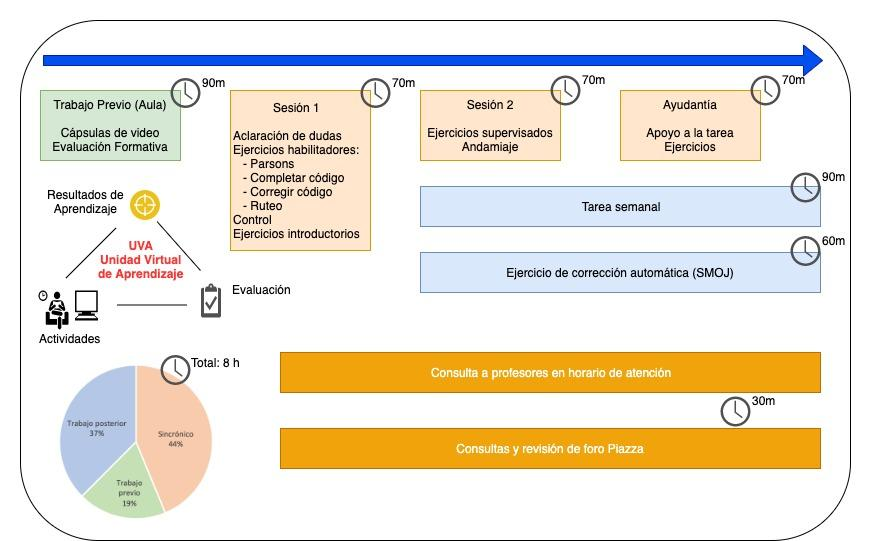
\includegraphics[width=1\textwidth]{uva.png}
  \caption{Modelo Formativo IWI-131. Fuente: Reglas del curso de programación de la UTFSM (2021-2).}
  \label{modeloiwi}
\end{figure}

Sin embargo, pese a que el curso cuenta con una gran cantidad de profesores, no son más de 5 los que se encargan de proponer tareas a la coordinación. Y, dado que cada semana se requiere una nueva tarea para la UVA en curso, se vuelve complicado elaborar tareas de calidad a tiempo, que cumplan con el alineamiento constructivista del curso, y que cuya resolución no requiera más tiempo que el estipulado en la UVA. Además, la elaboración de tareas se lleva a cabo sin métricas que permitan medir la calidad de cada una, o una metodología de elaboración de tareas que garantice la calidad de las mismas en el tiempo.

Entre los problemas que puede conllevar el uso de tareas que no son de calidad, se encuentran:

\begin{itemize}
  \item Pérdida del interés en aprender a programar \cite{10.1145/1227504.1227466}, de modo tal que el estudiante deje de ver el ramo como un curso de aprendizaje, y su actitud hacia él sea nétamente para aprobar.
  \item Frustración a lo largo del ramo, al punto en que el estudiante puede decidir desertar del curso y de la programación en general \cite{10.1145/2526968.2526982}.
  \item Aumentar las probabilidades de que los estudiantes realicen actos que falten a la honestidad académica para resolverla \cite{10.1145/3013499.3013507}.
  \item Complicar la elaboración de la rúbrica con la cual la tarea será evaluada, lo que puede conllevar a entregar un feedback menos valioso al estudiante
\end{itemize}

Es por esto que se requiere de un marco de trabajo que permita elaborar tareas de calidad, el cual brinde tanto una metodología como herramientas que faciliten a los profesores esta labor, ahorrándoles tiempo y garantizando a los estudiantes del curso una mejor experiencia de aprendizaje.

\subsection{Objetivos}

El objetivo general de esta memoria consiste en desarrollar un framework para la elaboración de tareas en cursos introductorios de programación.

\subsubsection{Objetivos Específicos}

Con el fin de lograr el objetivo general de esta memoria, se definen los siguientes como objetivos específicos de la misma:

\begin{itemize}
  \item Identificar y definir criterios que puedan ser usados para evaluar una tarea.
  \item Definir una métrica que permita evaluar una tarea de acuerdo al cumplimiento de criterios.
  \item Definir una metodología para la elaboración de tareas utilizando el framework Ishvel.
  \item Validar cómo la aplicación de la metodología definida elabora mejores tareas.
\end{itemize}

\begin{figure}[H]
  \centering
  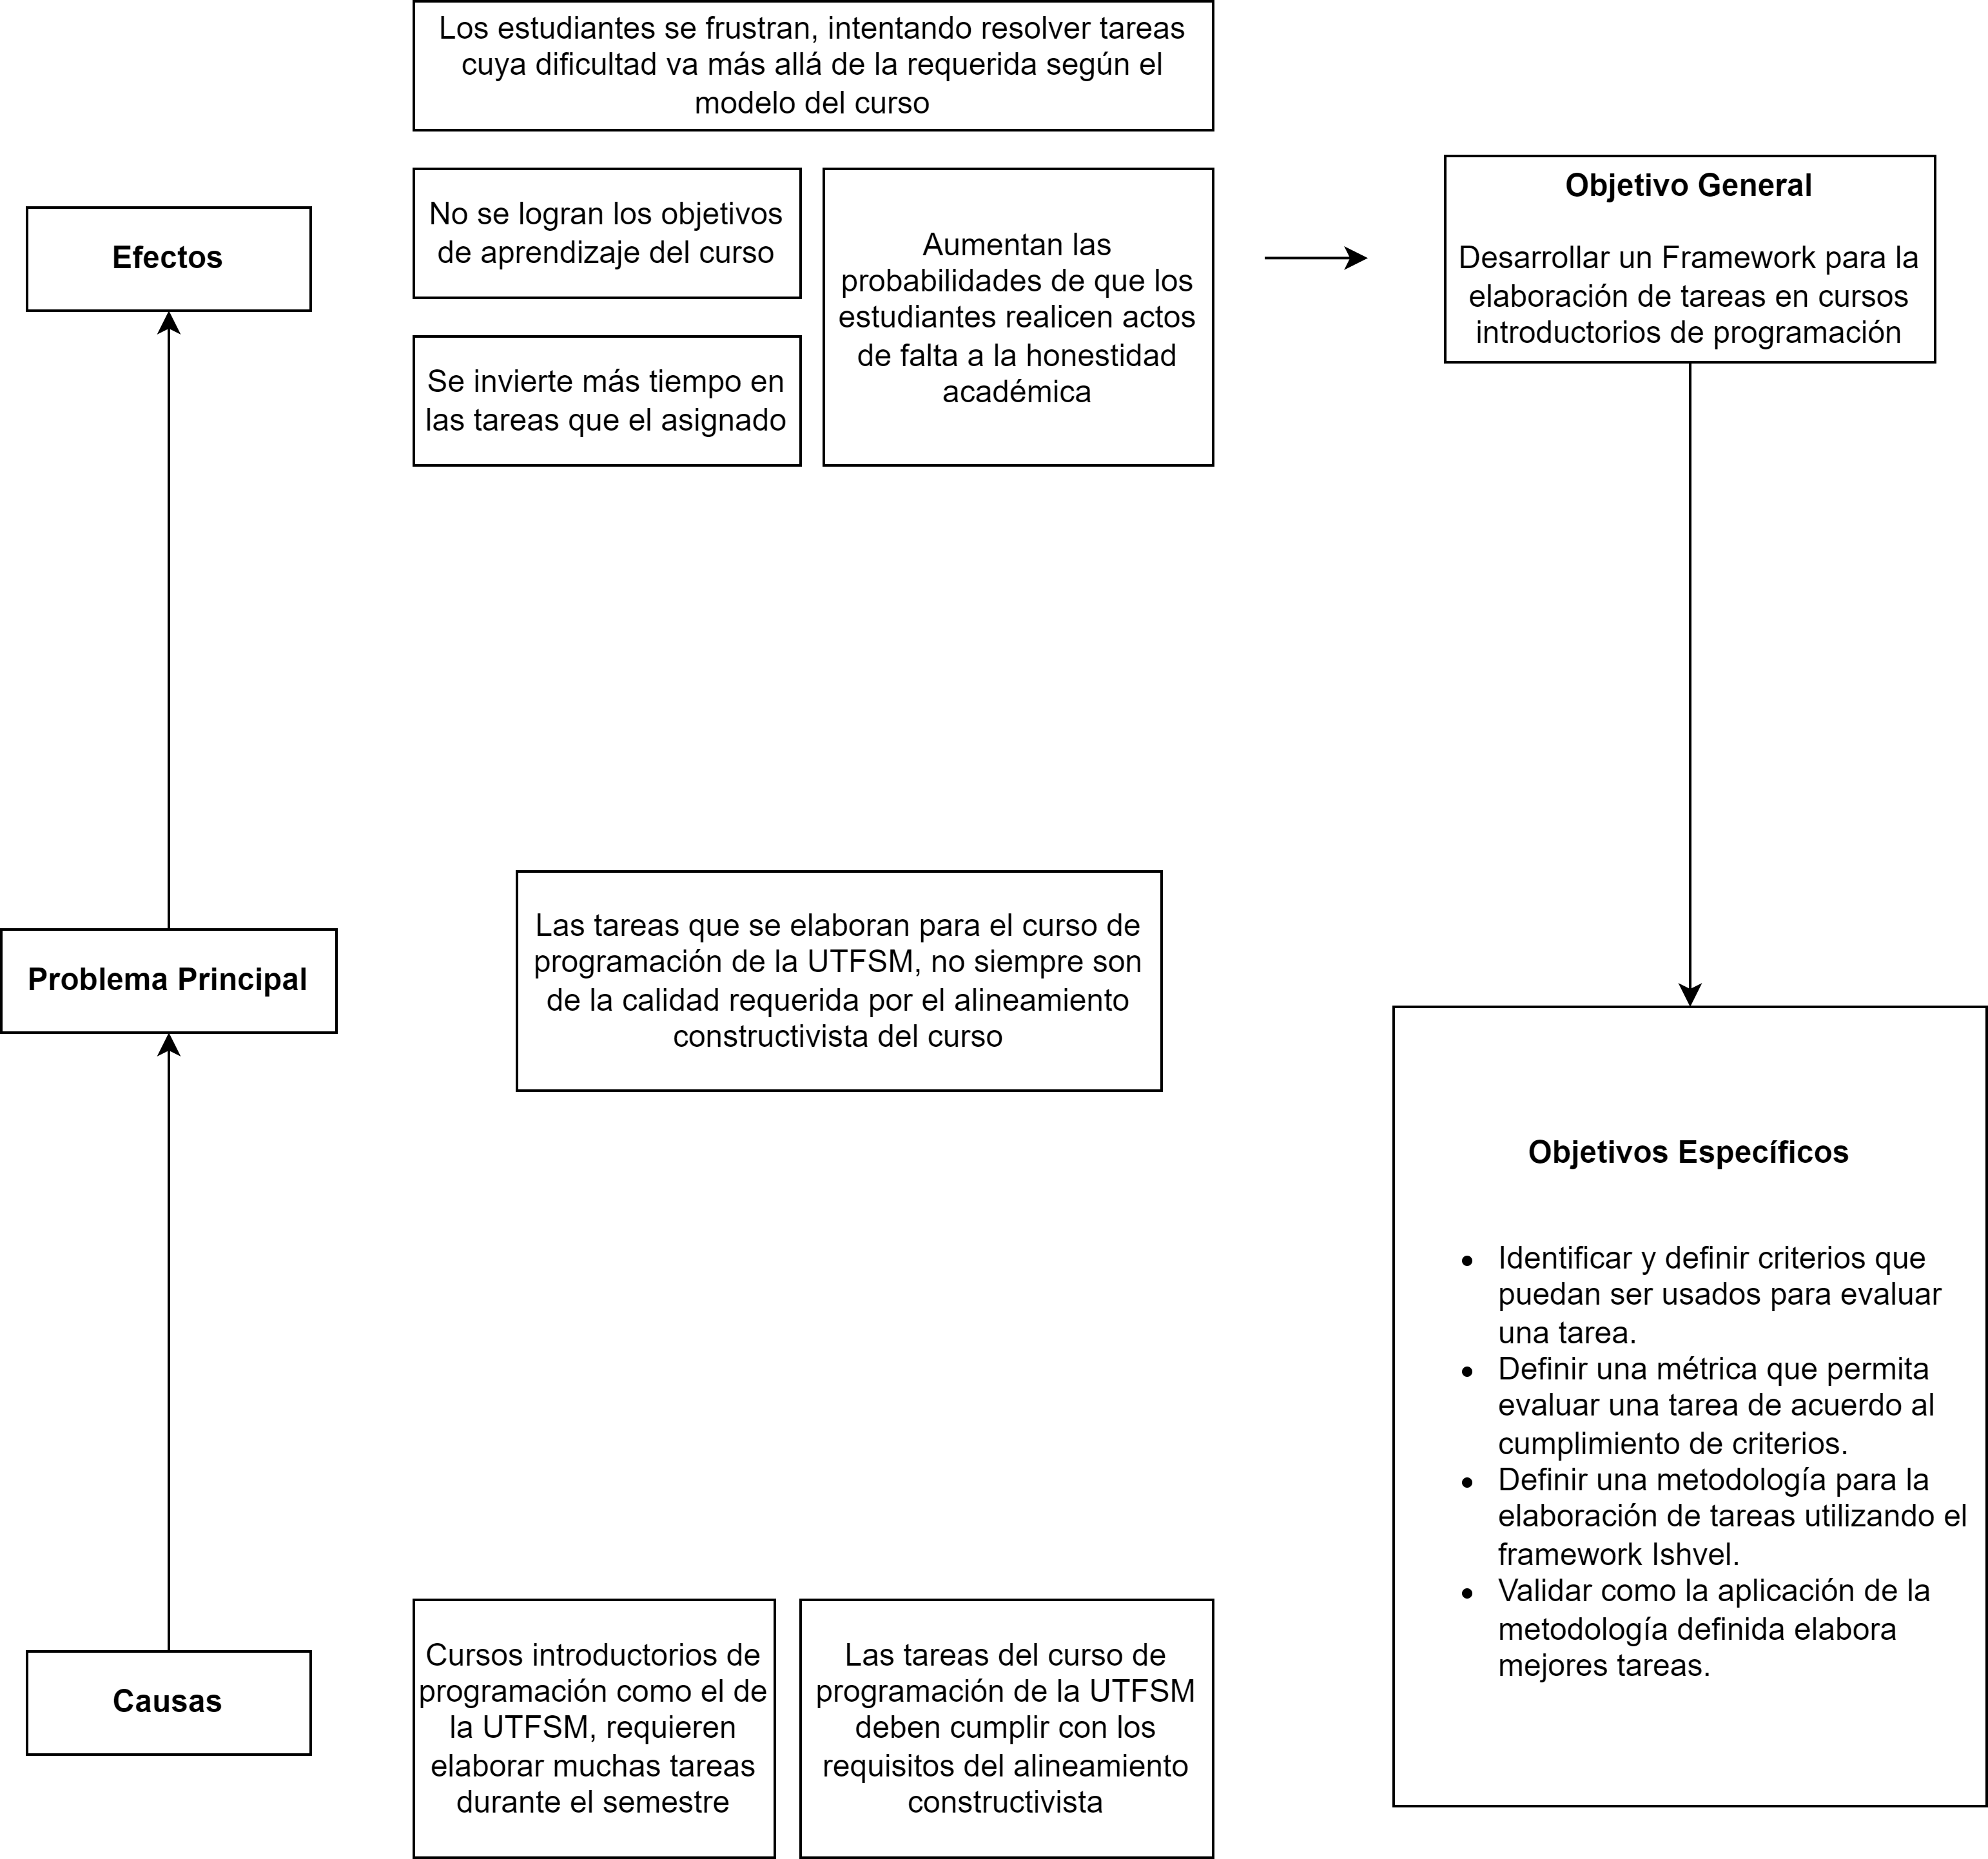
\includegraphics[width=1\textwidth]{arbolito.png}
  \caption{Árbol del Problema.} Fuente: elaboración propia.
  \label{arbolito}
\end{figure}

\newpage

\secnumbersection{MARCO CONCEPTUAL}

\subsection{Framework}

Un framework es un marco de trabajo \cite{la2012aprendizaje}, que plantea una metodología validada y un conjunto de herramientas, las cuales están diseñadas para la correcta aplicación de dicha metodología. Un framework se concibe en base a la acumulación de experiencia, buenas prácticas, patrones y soluciones validadas sobre el dominio de un problema recurrente, el cual ha sido abordado a través del tiempo y sus maneras de resolverse, han sido bien documentadas y mantenidas \cite{10.5555/326112}. A modo de ejemplo, en el área de la ingeniería de software, un framework brinda al desarrollador un esqueleto base para el desarrollo de algún software, el cual tiene como base la aplicación de distintos patrones arquitectónicos que permiten resolver de forma eficiente algún problema en particular \cite{elearn}.

\subsection{Sistemas de Gestión del Aprendizaje}


\subsection{Dominio de un Problema}

El dominio de un problema es un término de ingeniería para referirse a toda la información que define el problema, las restricciones de su solución, los objetivos que se desean lograr a la hora de abordarlo, el contexto donde el problema existe, y todas las reglas que definen la esencia del mismo. Este representa el entorno donde tanto el problema como sus soluciones propuestas se desenvuelven \cite{ProblemDomain}

\subsection{Frameworks en el Apoyo a la Enseñanza}

En el contexto de apoyar la labor de enseñar, los frameworks de este dominio apuntan a mejorar la gestión del contenido educativo, siguiendo buenas prácticas rescatadas del área de la ingeniería de software, y aplicadas al dominio de la enseñanza. Estas prácticas permiten reutilizar aspectos prácticos de un curso previo, como lo es su organización, sus contenidos, etc... y mejorarlos en el tiempo para así ahorrar tiempo y poder aplicar patrones de diseño que faciliten la labor de educar. A diferencia de los frameworks de ingeniería de software, estos frameworks están orientados a ser utilizados por un profesor, y en vez de entregar código, brindan herramientas y metodologías con las cuales el usuario puede gestionar de mejor manera su curso \cite{elearn}.

Por otro lado, al ser la enseñanza un dominio tan estudiado, existen muchos patrones que abordan diversas formas de resolver los problemas que ésta conlleva \cite{elearn}. Esta realidad ha impulsado enfoques que complementen los Sistemas de Gestión del Aprendizaje (LMS) con frameworks que recopilen patrones que apoyen la enseñanza, de este modo, si ya se cuenta con un curso cuya gestión es a través de un LMS como Moodle, entonces se puede implementar un framework sobre el LMS que permita integrar patrones adecuados para el desarrollo del curso (ver Figura \ref{patronlms}).

\begin{figure}[H]
  \centering
  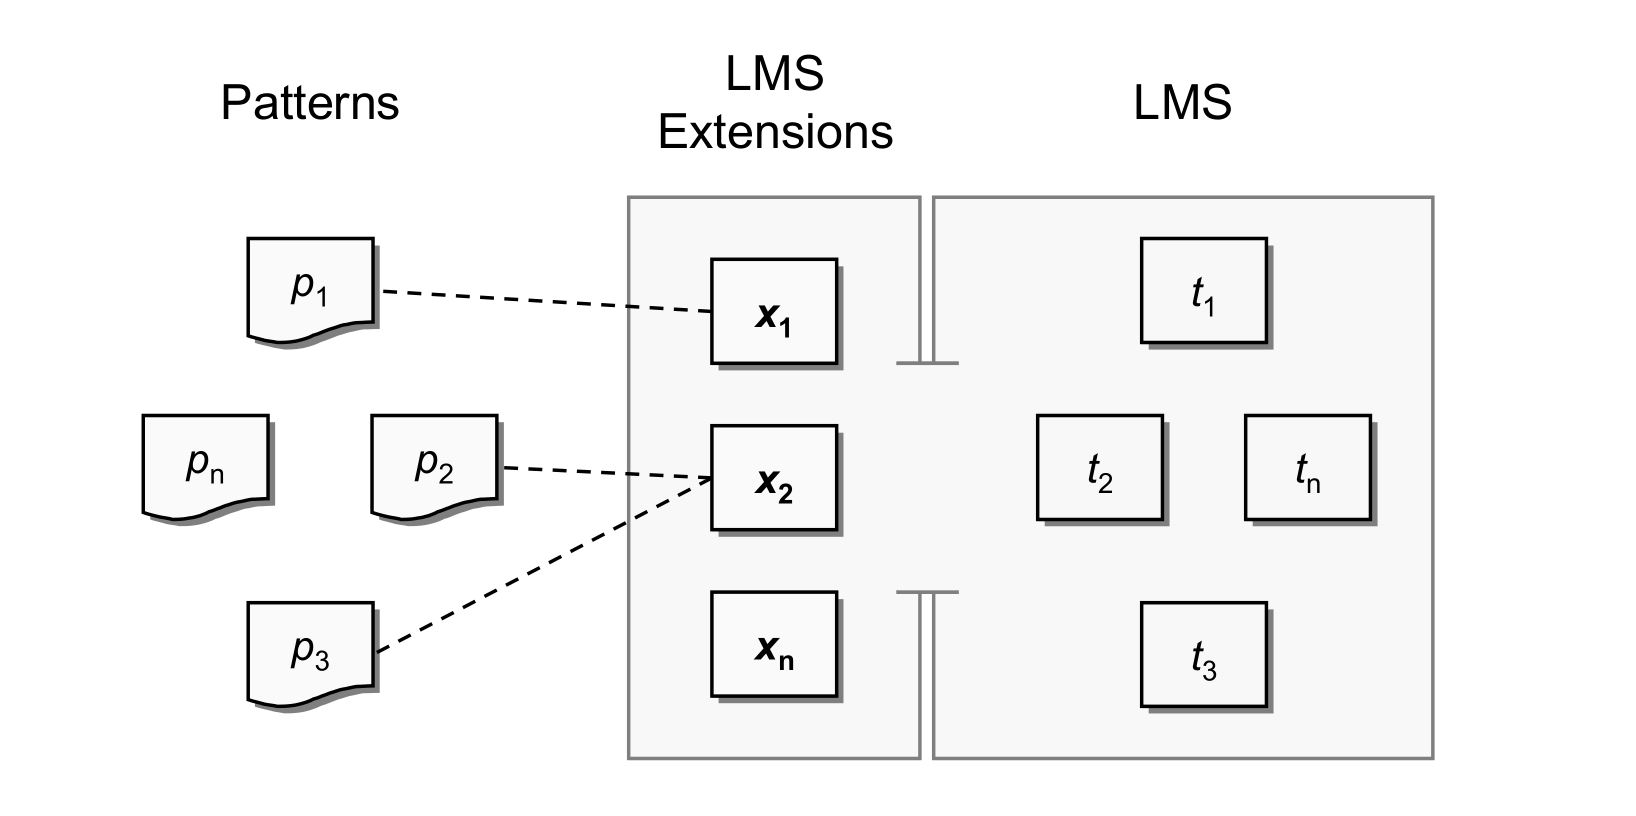
\includegraphics[width=1\textwidth]{patronlms.png}
  \caption{Implementación de los patrones de un framework en un LMS \cite{elearn}}
  \label{patronlms}
\end{figure}

Sin embargo, también existen enfoques donde el framework permite al profesor adaptar un conjunto de patrones, los cuales son seleccionados en base a la metodología de trabajo que el framework propone, para luego así hacer uso de ellos en la organización de un curso de manera controlada, lo cual garantiza que la metodología validada del framework se lleve a cabo de la manera más prolija. Ejemplo de esto es la interfaz del manejador de patrones de la herramienta CEWebS \cite{Mangler04cewebs} (ver Figura \ref{ceweb}).

\begin{figure}[H]
  \centering
  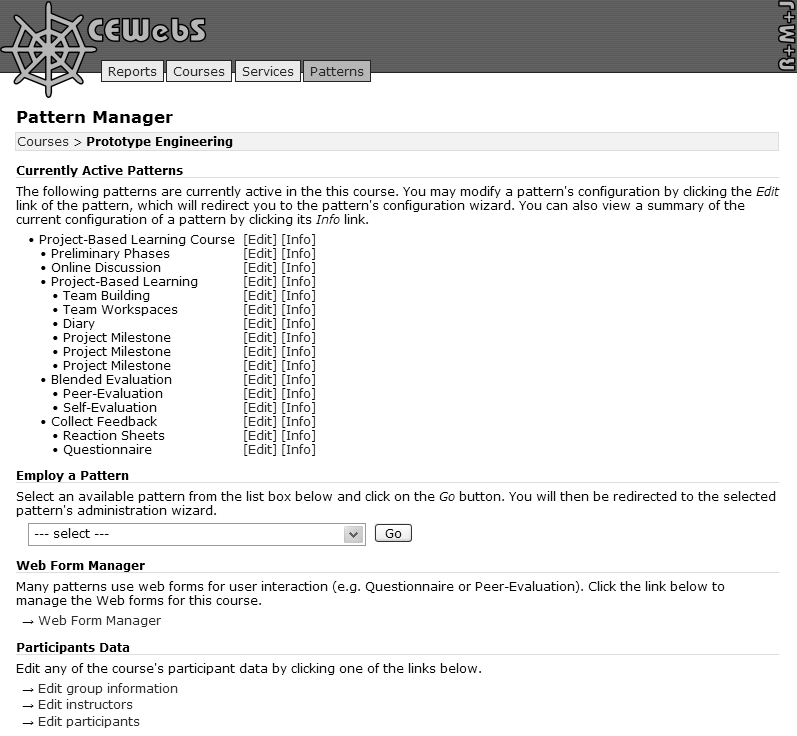
\includegraphics[width=1\textwidth]{ceweb.png}
  \caption{Pantalla principal de la interfaz de usuario de Patman (abreviación de \textit{pattern manager}) \cite{Mangler04cewebs}}
  \label{ceweb}
\end{figure}

Este último es la clase de framework que se implementará a lo largo de esta memoria, adaptándolo para la implementación de patrones adecuados y una metodología para la elaboración de tareas, de modo tal que guíe al profesor durante su uso, y garantice que éste siga una metodología adecuada para la tarea que está elaborando en el curso. Brindándole métricas de utilidad a medida que redacta, como una validación de que los objetivos de aprendizaje esperados para esa tarea, se cumplan en base a diversas validaciones, como lo sería la revisión del código que resuelve el problema, entre otros.

\subsection{Curso Introductorio de Programación}

Un cursos introductorio de programación es, en general, el primer acercamiento de un estudiante a los conceptos fundamentales de la computación \cite{10.7717/peerj-cs.647}, éstos tienen como enfoque entregar, a los estudiantes, los conceptos fundamentales de las ciencias de la computación, y son a su vez, cursos con altos niveles de reprobación, que pese a lo crucial que son en la formación del estudiante y de los futuros programadores, aún tienen muchos aspectos por mejorar en el tiempo, tanto en las tareas que tienen, como otros aspectos \cite{10.1145/2591708.2591749}. También son conocidos en la literatura y en diversos currículos universitarios como CS0 \cite{cs0} y CS1 \cite{cs1}, siendo CS2, CS3 y los que siguen,cursos que siguen la temática de las ciencias de la computación, pero que ya no tienen un caracter introductorio.

\subsection{Tarea de Programación}

Las tareas de programación son uno de los instrumentos con los cuales se evalúa, tanto los aprendizajes adquiridos de los estudiantes a lo largo del curso, como la puesta en práctica de los mismos. Generalmente constan de programar, sin embargo existen diversas adaptaciones según la forma en la que esté organizado el curso \cite{cs1}. Estas son el principal objeto de estudio de esta memoria, pues se busca lograr la elaboración de las mejores tareas posibles, en base al entendimiento del impacto que estas pueden tener en el estudiante, y en los indicadores de si una tarea es apropiada o no para llevarse a cabo en un curso introductorio de programación.

Diversos autores han abordado la elaboración y medición de tareas de calidad, enfocándose tanto en factores emocionales del estudiante \cite{10.1145/1839594.1839609, 10.1145/1227504.1227466, 10.5555/1968521.1968545, 10.1145/2526968.2526982}, como en aspectos particulares de cualquier tarea en sí \cite{texasU, 10.1145/2676723.2677276, 10.1145/1140124.1140167}. Y en general, siempre se destacan 3 aspectos principales:

\begin{itemize}
  \item Las tareas deben tener alguna aplicación real, o bien, resolver un problema real que le dé sentido al tiempo que el estudiante invertirá en resolverla.
  \item Las tareas deben ser interesantes, un problema puede expresarse utilizando un contexto de la actualidad, de lo que los estudiantes en general considerarían interesante como lo son sus bandas, juegos, tendencias, etc.
  \item Las tareas deben tener un nivel de dificultad adecuado, ni muy difíciles como para frustrar al estudiante, ni muy fáciles como para no cumplir con los objetivos de aprendizaje de la misma.
\end{itemize}

\subsubsection{Factores de Importancia en una Tarea de Programación}

Un estudio acerca de los factores que despiertan el interés e impulsan la elección de un estudiante en el desarrollo de una tarea, indica que en el caso del interés, los factores que más interés generan de una tarea son (en orden decreciente de importancia):

\begin{itemize}
  \item Que tenga gráficos
  \item Que tenga alguna utilidad en el mundo real
  \item Que sea entretenida
  \item Que sea desafiante
  \item Que sea fácil
  \item Que se relacione con algún hobby
\end{itemize}

Mientras que en los factores que llevarían a un estudiante a elegir desarrollar una tarea por sobre otra, se encuentran (en orden decreciente de importancia):

\begin{itemize}
  \item Que sea fácil
  \item Que tenga alguna utilidad en el mundo real
  \item Que sea entretenida
  \item Que sea desafiante
  \item Que se relacione con algún hobby
  \item Que tenga gráficos
\end{itemize}

Estos factores se resumen en el siguiente gráfico (ver Figura \ref{elecciones})

\begin{figure}[H]
  \centering
  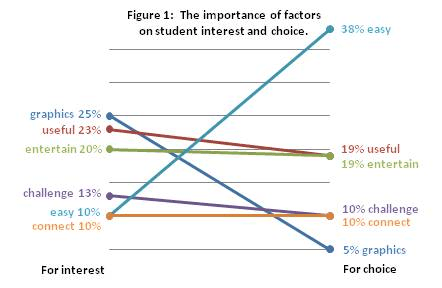
\includegraphics[width=1\textwidth]{elecciones.png}
  \caption{Nivel de importancia de los factores de una tarea, asignado por los mismos estudiantes según si les genera interés, o si les haría elegir desarrollar esa tarea por sobre otra \cite{10.5555/1968521.1968545}}
  \label{elecciones}
\end{figure}

\subsubsection{Reutilización de Tareas de Programación}

La imperante necesidad de tener tareas nuevas cada semestre para un curso (pese a los cambios que la pandemia ha conllevado en algunos \cite{10.1145/3456565.3461439}), ha impulsado la investigación respecto a como reutilizar de forma eficiente las tareas de semestres anteriores \cite{10.1145/3477429}, sin embargo, proyectos como Moulinog \cite{10.1145/3414080.3414100} han sido muy limitados en lograr esto, pues están limitados a, en base a 1 tarea, generar múltiples tareas que son en esencia lo mismo con la salvedad de cambiar ciertos valores y palabras, que no garantizan que 1 misma solución no sea esencialmente capaz de resolver 2 tareas distintas de las generadas.

Sin embargo, la idea de tener tareas base motiva a investigar acerca de si es buena idea re-utilizar tareas, generando un pequeño banco de tareas de calidad, pero teniendo en cuenta que éstas deben ser del tipo \textit{Tweakable assignments} \cite{10.1145/3477429}, es decir, la mayoría de sus partes pueden re-utilizarse, a excepción de algunas que, en base a ciertas especificaciones, deben modificarse en la nueva tarea de modo tal que una solución a la tarea original, simplemente no funcione con la tarea nueva que se está elaborando, manteniendo así la calidad de la tarea original, y evitando llegar a aumentar las probabilidades de actos fraudulentos por parte de los estudiantes, quienes pueden hacerse de las soluciones de tareas anteriores \cite{10.1145/3013499.3013507}.

\subsection{Métricas de Software}

Las métricas de software son valores computados con el objetivo de evaluar ciertas características del software desarrollado\cite{1702275}. Existen diversas métricas de software las cuales se concentran en distintos aspectos del mismo, a continuación se explican las más relevantes para esta investigación.

\subsection{Complejidad Ciclomática}

La complejidad ciclomática es una métrica de software creada por Thomas McCabe, la cual mide el número de caminos linealmente independientes a través de una porción de código\cite{7725232}. Hoy en día es una de las métricas más utilizadas en la industria para determinar la complejidad de entender y mantener un código, así como también la probabilidad de que éste tenga defectos. Un alto valor de esta métrica implica una densidad de defectos a lo largo de él, así como también, da cuenta de la cantidad de decisiones distintas que el programa debe tomar, y por tanto, lo complejo que es entender el problema subyacente que se intenta resolver.

La complejidad ciclomática de un programa se calcula mediante su grafo de ejecución, donde cada línea de código corresponde a un nodo del grafo, y cada nodo tendrá una arista hacia el nodo que sigue inmediatamente según la línea de ejecución del código. Una vez que está hecho el grafo de ejecución, la fórmula para la complejidad ciclomática es:

\begin{equation}
  CC = E - N + 2P
\end{equation}

Donde:

\begin{itemize}
  \item $CC$: Complejidad Ciclomática
  \item $E$: Cantidad de aristas del grafo de ejecución
  \item $N$: Cantidad de nodos del grafo de ejecución
  \item $P$: Cantidad de componentes conexas del grafo
\end{itemize}

\subsection{Métricas de Halstead}

Maurice H. Halstead propuso una serie de métricas de software en su libro ``Elements of Software Science'' \cite{10.5555/540137}, las cuales buscaban predecir de manera experimental como el hecho de escribir código también es una ciencia governada por leyes naturales. No obstante, en el futuro se realizaron experimentos que demuestran que el trabajo propuesto no representa realmente ninguna ley natural \cite{10.5555/800254.807762}, aún así, éstas métricas han sido ampliamente utilizadas en la industria para medir la mantenibilidad de su software.

Halstead inicia su obra definidiendo los siguientes parámetros para la implementación en código de cualquier algoritmo:

\begin{itemize}
  \item $\eta_{1}$: Número de \textit{operadores} únicos que aparecen en la implementación
  \item $\eta_{2}$: Número de \textit{operandos} únicos que aparecen en la implementación
  \item $N_{1}$: Uso total de todos los \textit{operadores} que aparecen en la implementación
  \item $N_{2}$: Uso total de todos los \textit{operandos} que aparecen en la implementación
  \item $f_{1,j}$: Número de ocurrencias del $j$-ésimo \textit{operador} más frecuente en la implementación, donde $j = 1, 2, ..., \eta_{1}$
  \item $f_{2,j}$: Número de ocurrencias del $j$-ésimo \textit{operando} más frecuente en la implementación, donde $j = 1, 2, ..., \eta_{2}$
\end{itemize}

De estos parámetros, se definen el vocabulario $\eta$ de la implementación como:
\begin{equation*}
  \eta = \eta_{1} + \eta_{2}
\end{equation*}
Y el largo $N$ de la implementación como:
\begin{equation*}
  N = N_{1} + N_{2}
\end{equation*}
Basado en esto, Halstead plantea las siguientes métricas:

\subsubsection{Volumen de un Programa}

Una característica importante de la implementación de cualquier algoritmo es su tamaño, sin embargo, a medida que la implementación de éste es traducida de un lenguaje de programación a otro, su tamaño cambia. Por lo tanto, una métrica de tamaño que sólo considere la cantidad de caracteres de la implementación, no será suficientemente objetiva dado la diferencia de caracteres que pueden tener operandos u operadores similares en lenguajes de programación distintos.

Para abordar este problema, se debe notar que para cualquier implementación, existe un mínimo largo absoluto con el cual se puede representar el operador u operando más largo utilizado, éste mínimo es la representación en bits del mismo. El largo dependerá sólo de la cantidad de elementos en el vocabulacio del programa, es decir, $\eta$. Por ejemplo, para $\eta = 8$ se requieren sólo 3 bits con los cuales se puedan representar todos los elementos del vocabulario, y a modo general, se requieren $\log_{2}\eta$ bits para representar en su largo mínimo cualquiera de los elementos de un programa.

Esta interpretación nos entrega una dimensión en bits del volumen de cualquier programa, y permite medir el tamaño de cualquier implementación para cualquier algoritmo definiendo el \textit{volumen} $V$ como:
\begin{equation}
  V = N\log_{2}\eta
\end{equation}
\subsubsection{Volumen Potencial}

Dado que al traducir la implementación de un algoritmo de un lenguaje a otro, implicará un cambio en el volumen del programa, se requiere otra métrica que de cuenta de la mínima forma en la que se puede expresar un algoritmo. Por ejemplo, si un lenguaje de programación ya cuenta con la subrutina o procedimiento que implementa un algoritmo, sólo se requiere llamarla y entregarle los parámetros correspondientes.

Para este caso, si se denotan los parámetros en su forma mínima absoluta, se puede definir que la mínima forma de implementación de cualquier algoritmo, nombrado de ahora en adelante como \textit{volumen potencial V*}, es:
\begin{equation}
  \label{eqn:potentialVolume}
  V^{*} = (N_{1}^{*} + N_{2}^{*}) \cdot \log_{2}(\eta_{1}^{*} + \eta_{2}^{*})
\end{equation}
Donde:
\begin{itemize}
  \item $V^{*}$: Volumen potencial
  \item $N_{1}^{*}$: Mínimo uso total de operadores de la implementación
  \item $N_{2}^{*}$: Mínimo uso total de operandos de la implementación
  \item $\eta_{1}^{*}$: Mínima cantidad de operadores únicos de la implementación
  \item $\eta_{2}^{*}$: Mínima cantidad de operandos únicos de la implementación
\end{itemize}
Dado que en la forma mínima, no se requiere repetición de operandos ni operadores, entonces:
\begin{equation*}
  N_{1}^{*} = \eta_{1}^{*}
\end{equation*}
\begin{equation*}
  N_{2}^{*} = \eta_{2}^{*}
\end{equation*}
Además, según lo planteado anteriormente, el mínimo número de operadores a utilizar serán sólo un operador para invocar a la subrutina o procedimiento, y otro para almacenar el resultado de la misma, por lo tanto:
\begin{equation*}
  \eta_{1}^{*} = 2
\end{equation*}
Con esto la ecuación \ref{eqn:potentialVolume} queda como:
\begin{equation}
  V^{*} = (2 + \eta_{2}^{*}) \cdot \log_{2}(2 + \eta_{2}^{*})
\end{equation}
Donde $\eta_{2}^{*}$ debería representar el número de distintos parámetros de input y output de la subrutina o procedimiento. Con esto, $V^{*}$ es independiente del lenguaje en cual se exprese cualquier algoritmo, por lo tanto a diferencia de $V$, $V^{*}$ no cambiará al traducir un algoritmo de un lenguaje a otro.

\subsubsection{Nivel de un Programa} \label{sssec:programLevel}

Existe de manera intuitiva una idea del ``nivel'' que un programa tiene, el cual es determinado en base a la opinión de un grupo de expertos, basándose en que el nivel de un programa tiene un impacto en el esfuerzo de escribirlo, cometer errores en él y la facilidad con que puede entenderse. Sin embargo, esta métrica no puede quedar como una opinión, y con el fin de llevarla a algo cuantitativo, se propone la siguiente definición para el \textit{nivel de un programa} $L$ como:
\begin{equation}
  \label{eqn:programLevel}
  L = \frac{V^{*}}{V}
\end{equation}
Lo que indica que la versión mínima en la que se puede escribir un algoritmo tendrá un nivel de 1, otras implementaciones con un mayor volumen un nivel menor, lo que implica que $L \leq 1$. Es importante notar que si se aplica esta métrica para evaluar qué tan fácil o difícil es entender un programa, ocurre que para una persona con un alto entendimiento del lenguaje de programación utilizado, será muy sencillo entender un programa con un bajo volumen, lo que conllevaría a que tenga un alto nivel, por otro lado, para una persona menos fluída en el mismo lenguaje, será más sencillo entender un programa con un mayor volumen, lo que implicará un menor nivel de programa. Dicho esto, se plantea que la dificultad de entender un programa es inversamente proporcional al nivel del mismo.

Sin embargo, dada la ausencia de un valor conocido para el volumen potencial de una implementación (debido a que no existe un lenguaje de programación que implemente todos los algoritmos como subrutinas o procedimientos), es preferible obtener un cálculo del nivel del programa directamente de la implementación, sin hacer referencia a una posible subrutina que permita implementar el algoritmo en su forma mínima. Esto puede lograrse notando como impactan por separado los operadores y operandos en el nivel del programa.

El menor nivel de operadores que se puede utilizar es 2 (la invocación de una subrutina o procedimiento, y un operador para asignar su resultado en alguna variable), por otro lado, no hay un límite de la cantidad de operadores únicos que pueden haber, de aquí se desprende que:
\begin{equation}
  \label{eqn:programLevel1}
  L \approx \frac{\eta_{1}^{*}}{\eta_{1}}
\end{equation}
Por otro lado, no existe un mínimo para los operandos, a su vez, el que se repita mucho un mismo operando apoya a que el nivel del programa sea bajo. Este efecto puede medirse en base al radio del uso total de operandos únicos en la implementación, de donide se obtiene la segunda proporcionalidad:
\begin{equation}
  \label{eqn:programLevel2}
  L \approx \frac{\eta_{2}}{N_{2}}
\end{equation}
Combinando las ecuaciones \ref{eqn:programLevel1} y \ref{eqn:programLevel2}, se obtiene una versión alternativa para el cálculo del nivel de un programa.
\begin{equation}
  \label{eqn:programLevel3}
  \hat{L} = \frac{\eta_{1}^{*}}{\eta_{1}} \cdot \frac{\eta_{2}}{N_{2}}
\end{equation}
Y sabiendo que $\eta_{1}^{*}$, la ecuación queda como:
\begin{equation}
  \label{eqn:programLevel4}
  \hat{L} = \frac{2}{\eta_{1}} \cdot \frac{\eta_{2}}{N_{2}}
\end{equation}
La experimentación muestra que ambas ecuaciones son aceptables, sin embargo a lo largo de este documento se utilizará la ecuación \ref{eqn:programLevel4}.

\subsubsection{Dificultad de un Programa}

La dificultad de un programa según Halstead, es el inverso del nivel del mismo, entonces basándose en lo planteado en la sección \ref{sssec:programLevel}, se define la dificultad de un programa $D$ como:
\begin{equation}
  D = \frac{1}{\hat{L}} = \frac{\eta_{1}}{2} \cdot \frac{N_{2}}{\eta_{2}}
\end{equation}

\subsubsection{Esfuerzo de Programación}

El esfuerzo de desarrollar un programa dado corresponde a la actividad mental requerida para escribirlo, ésta fórmula se desprende de la siguiente manera:

\begin{enumerate}
  \item Se debe asumir que cualquier implementación de cualquier algoritmo, consiste en realizar $N$ selecciones de un vocabulario de $\eta$ elementos.
  \item El cerebro es eficiente a la hora de realizar búsquedas, por lo tanto, se puede decir que es equivalente a hacer una búsqueda binaria, lo que implica que el cerebro realiza $\log_{2}\eta$ comparaciones para la selección de cada uno de los elementos de la implementación.
  \item En base a los puntos anteriores, se puede determinar que un programa es generado mediante la realización de $N \cdot \log_{2}\eta$ comparaciones mentales.
  \item Recordando que el volumen de un programa se define como $V = N\log_{2}\eta$, se determina que el volumen de un programa es también un contador del número de comparaciones mentales requeridas para generar un programa.
  \item Cada comparación mental requiere un número de discriminaciones mentales, es decir, de descartar algunos elementos del vocabulario que no corresponden a lo que se busca implementar durante la búsqueda binaria del elemento correcto. Este número de discriminaciones mentales equivale a la dificultad de la tarea a realizar, y refuerza la idea de que el nivel de programación $L$ es recíproco a la dificultad de programación.
  \item Habiendo determinado que $V$ equivale a la cantidad de comparaciones mentales a realizar, y el recíproco del nivel de programación $\frac{1}{L}$ es una medida del promedio de discriminaciones mentales requeridas para cada comparación, es posible plantear que el número total de discriminaciones mentales $E$ requeridas para generar un programa es:
        \begin{equation}
          E = \frac{V}{L}
        \end{equation}
  \item Recordando de la ecuación \ref{eqn:programLevel}, se puede reemplazar $L$ por $\frac{V^{*}}{V}$, obteniendo así que la fórmula del esfuerzo de programación se puede ver como:
        \begin{equation}
          \label{eqn:programEffort}
          E = \frac{V^{2}}{V^{*}}
        \end{equation}
\end{enumerate}
Con esto se obtiene que el esfuerzo mental requerido para la implementación de cualquier algoritmo, está cuadráticamente relacionado con el volumen del mismo.

\subsubsection{Tiempo Estimado de Programación}

Según el trabajo de John Stroud en su obra ``The Fine Structure of Psychological Time'' \cite{https://doi.org/10.1111/j.1749-6632.1967.tb55012.x}, existe una cantidad de tiempo requerido por el cerebro humano para realizar una discriminación de elementos, y que por lo tanto, existe una cantidad de discriminaciones que puede hacer por segundo. De aquí nace el número de Stroud $S$, el cual indica los límites para la cantidad de discriminaciones por segundo que puede hacer el cerebro humano, y está acotado por:
\begin{equation}
  5 \leq S \leq 20
\end{equation}
Dado que la cantidad de discriminaciones que el cerebro humano puede hacer, está limitada por los límites del número de Stroud, y que la ecuación \ref{eqn:programEffort} del esfuerzo de programación tiene dimensiones de dígitos binarios por cantidad de discriminaciones, es posible estimar el tiempo en que un ser humano tardaría en realizar la implementación de un algoritmo como:
\begin{equation}
  T = \frac{E}{S}
\end{equation}
Donde S será considerado 18 según los experimentos de Halstead.

\newpage

\secnumbersection{PROPUESTA DE SOLUCIÓN}

\subsection{Historias de Usuario}

\subsection{Herramientas y Tecnologías a Utilizar}

El framework consiste de una serie de tecnologías y herramientas utilizadas tanto para la aplicación de la metodología, como para el desarrollo y funcionamiento de la aplicación para editar y evaluar tareas. Estas herramientas y tecnologías se listan a continuación:

\subsubsection{WebAssembly}

Es un formato binario de instrucciones para una máquina virtual basa en pilas, diseñado para ser un punto de compilación portable para distintos lenguajes de programación. Esta tecnología permite desplegar programas en diferentes lenguajes tanto en aplicaciones de cliente como de servidor \cite{WebAssemblyCoreSpecification2}.

Gracias a WebAssembly, es posible ejecutar una biblioteca de Python en una aplicación en Javascript para ser utilizada en el navegador, sin tener que instalar programas extras ni realizar configuraciones tediosas en el navegador del usuario.

\subsubsection{Python}

Es un lenguaje de programación interpretado fácil de aprender, con eficientes estructuras de datos de alto nivel y un enfoque simple pero efectivo hacia la programación orientada a objetos \cite{PythonWebsite}. Consta de múltiples módulos y es ampliamente utilizado en la industria para el desarrollo de aplicaciones.

Las tareas del curso IWI-131 de programación de la Universidad Técnica Federico Santa María deben ser resueltas en este lenguaje, y es a su vez el lenguaje principal que se estudia en el presente trabajo.

\subsubsection{Javascript}

Es un lenguaje de programación interpretado basado en prototipos, multiparadigma y de un único hilo. Es uno de los lenguajes de scripting más conocidos para el desarrollo web, pero también es utilizado ampliamente en la industria para otro tipo de aplicaciones y ambiantes \cite{MDNJavaScript}.

Su uso en conjunto con WebAssembly permite el desarrollo de aplicaciones de navegador que utilizan distintos lenguajes de programación a la vez, como por ejemplo, Python con Javascript.

\subsubsection{Markdown}

Es una herramienta de conversión de texto plano a HTML para creadores de contenido web, éste permite crear textos en un formato sencillo de leer y escribir, para luego ser convertido en un código estructuradamente válido de HTML \cite{DFMarkdown}.

Con Markdown es posible estructurar la redacción de distintos tipos de artículos, entre éstos, tareas de programación, lo que facilita su creación, distribución y estandarización a lo largo de las distintas personas que trabajan en la redacción de las mismas.

\subsubsection{GitHub Pages}

Es un ambiente provisto por Github$\texttrademark$ para desarrollar y publicar sitios web, haciendo posible alojar un sitio web estático de forma fácil, rápida y gratuita \cite{Utomo_2020}. Con esto, es posible delegar la responsabilidad de alojar una aplicación web a Github$\texttrademark$, y así no tener que contar con un servidor propio el cual deba ser manualmente mantenido.

\subsubsection{Multimetric}

Es una librería de Python para calcular métricas de código para programas en distintos lenguajes de programación \cite{privkweihmann_multimetric}. Entre las métricas que calcula esta librería se encuentran:

\begin{itemize}
  \item Complejidad ciclomática
  \item Dificultad según Halstead
  \item Esfuerzo según Halstead
  \item Tiempo estimado de programación según Halstead
  \item Volumen según Halstead
\end{itemize}

\subsubsection{Pyodide}

Es una versión de Python y una colección de distintos módulos de python compilados a WebAssembly. Este proyecto ha llevado exitósamente el intérprete de Python a un módulo de WebAssembly, permitiendo así que un código de Python sea executado sin problemas en un navegador web \cite{huffman2023julia}. Multimetric es una de las librerías que puede ser ejecutada en un navegador gracias a este módulo.

\subsubsection{React}

Es un framework de Javascript, originalmente creado por Facebook$\texttrademark$ para resolver los problemas de desarrollar interfaces de usuario complejas con datos que cambian en el tiempo. React cambió la forma en que las aplicaciones eran creadas logrando enormes avances en como se lleva a cabo el desarrollo web \cite{Gackenheimer2015}.

\subsection{Arquitectura de la Solución}

\subsubsection{Sistema de Software Autocontenido}

\subsection{Framework}

El marco de trabajo de Ishvel se propone con el fin de entregar una herramienta docente, la cual permite obtener una noción de la dificultad de una tarea antes de ésta ser entregada al estudiantado para su resolución, para ello, Ishvel se basa en el código que resuelve la tarea de manera correcta, extrayendo métricas del mismo y comparándolas con las métricas de tareas anteriores.

\subsubsection{Metodología}

Ishvel ofrece un acercamiento a entender la dificultad de una tarea en comparación a tareas anteriores, antes de publicar la misma a los estudiantes. Para esto, se la siguiente metodología de trabajo:

\begin{itemize}
  \item Desde el editor de Ishvel, seleccionar las configuraciones adecuadas para el contenido de la tarea que se va a desarrollar, y el semestre y tipo de soluciones con la cual compararla. Para esto, se ofrecen las siguientes opciones:
        \begin{itemize}
          \item \textbf{Contenido de la tarea}: Opción para determinar de qué contenido será la tarea a elaborar, lo que configura el editor para utilizar las métricas de tareas anteriores del contenido seleccionado
          \item \textbf{Semestre a comparar}: Opción para determinar de qué semestre serán las tareas del contenido seleccionado las que se utilizarán para comparar
          \item \textbf{Tareas a comparar}: Opción para determinar si las métricas de la tarea a elaborar se compararán con las métricas de las soluciones de los profesores o de los estudiantes, del semestre seleccionado previamente.
        \end{itemize}
        \begin{figure}[H]
          \centering
          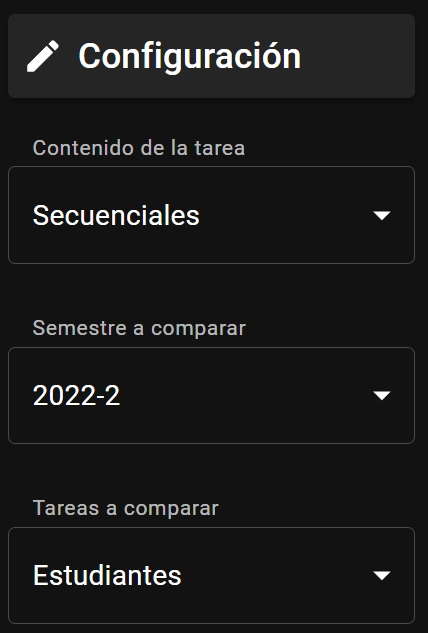
\includegraphics[width=0.4\textwidth]{figures/ishvel1.png}
          \caption{Opciones de configuración del editor de Ishvel.} Fuente: elaboración propia.
          \label{img:ishvel1}
        \end{figure}
  \item Una vez configurado el editor, iniciar por el título de la tarea, añadir alguna imagen representativa, y proceder a seguir el formato de ejemplo del editor:
        \begin{itemize}
          \item \textbf{Contexto}: Contextualización corta reapecto al problema que se está enfrentando, buscando que sea real, concisa e interesante. En caso de necesitar ideas para contextualizar el problema, se puede ver la \textit{sugerencia por defecto} que el framework ofrece, la cual invita al docente a abrir Google Trends $\texttrademark$ y ver situaciones de actualidad que pueden ser interesantes para el contexto de un problema.
                \begin{figure}[H]
                  \centering
                  
\includegraphics[width=0.8\textwidth]{figures/ishvel2.png}
                  \caption{Sugerencia inicial del editor de Ishvel.} Fuente: elaboración propia.
                  \label{img:ishvel2}
                \end{figure}
          \item \textbf{Instrucciones}: Sección con la lista de instrucciones de lo que el estudiante debe realizar, concentrándose en que éste pueda relacionar lo que el texto dice con lo que él debe escribir en su programa. La idea de separar la sección de instrucciones de la sección de contextualización, es poder tener un espacio centrado nétamente en cómo el estudiante traducirá instrucciones en lenguaje humano a lenguaje máquina, sin tener distractores o tener que pasar por algún proceso cognitivo previo del cual desprender lo que se debe hacer, como lo sería por ejemplo mezclando el contexto con las instrucciones en un sólo texto.
          \item \textbf{Ejemplos}: Sección con ejemplos de la salida completa del programa, de esta manera, el estudiante tiene una guía visual de cómo debería ser su programa, y no tiene que imaginar por completo los detalles visuales de la salida del programa, para así concentrarse en programar.
          \item \textbf{Recomendaciones}: Sección extra con las recomendaciones que se pueden dar al estudiante para que realice un mejor trabajo, así como también, restricciones al mismo con las cuales el estudiante evite utilizar herramientas o librerías que no están consideradas como parte de lo que se busca evaluar en la tarea.
        \end{itemize}
        \begin{figure}[H]
          \centering
          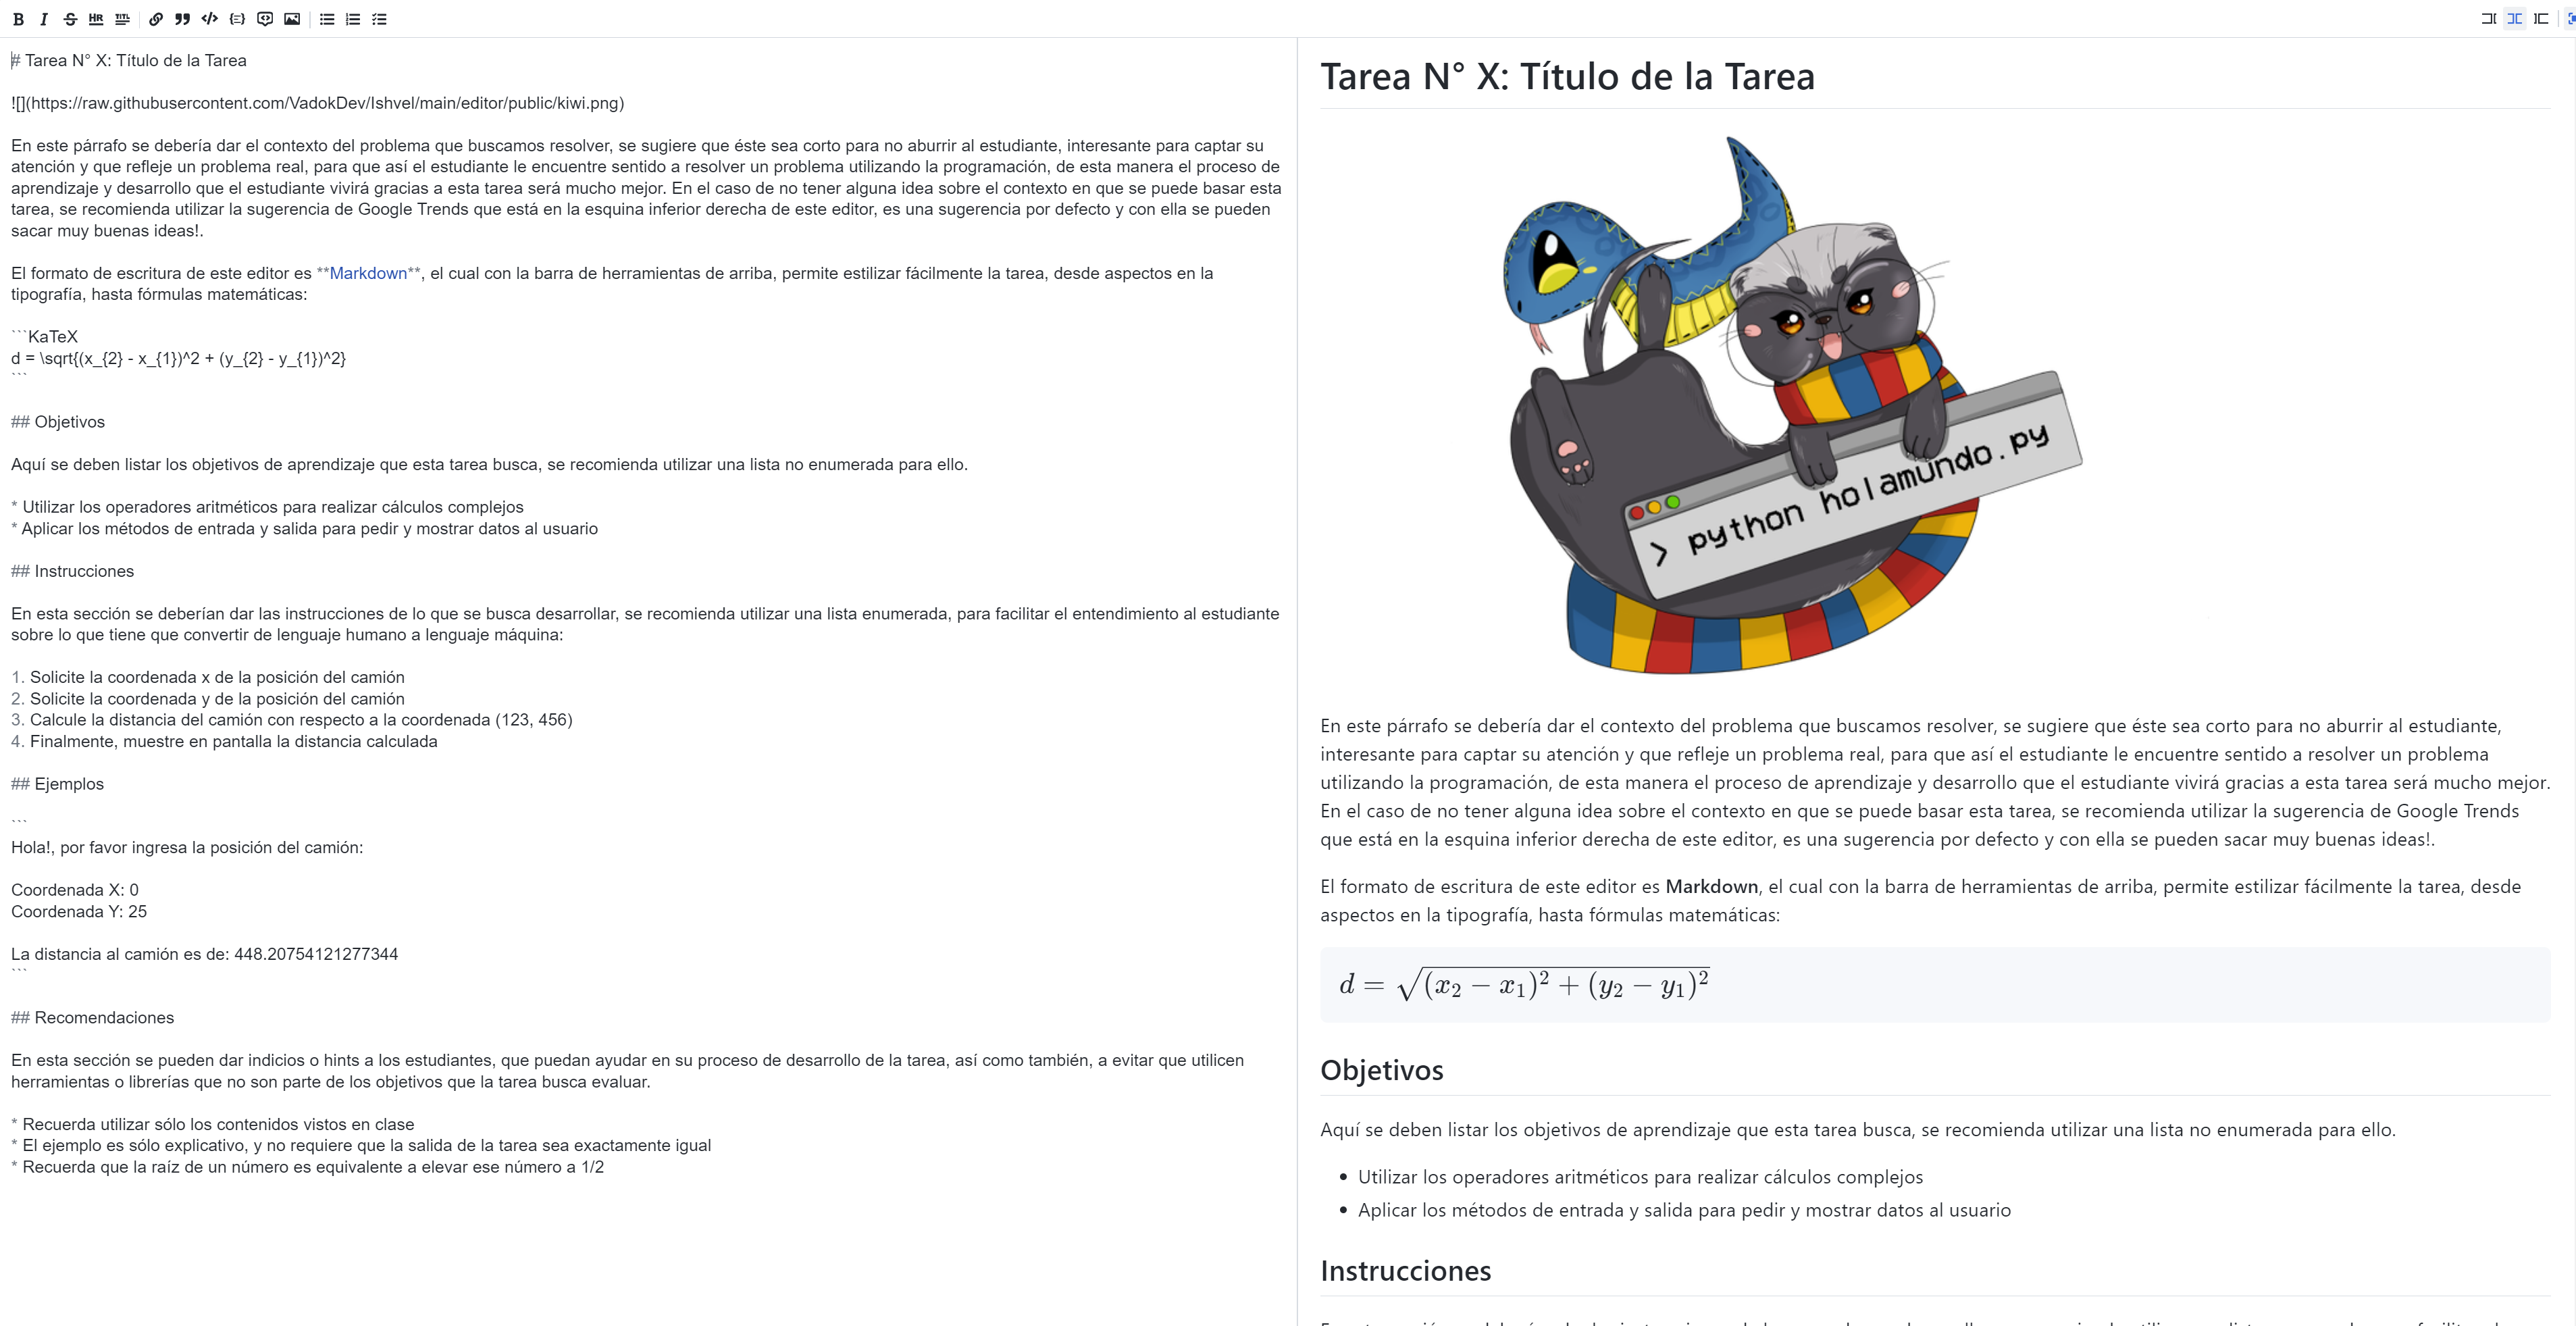
\includegraphics[width=1\textwidth]{figures/ishvel8.png}
          \caption{Formato de ejemplo de una tarea en el editor de Ishvel.} Fuente: elaboración propia.
          \label{img:ishvel3}
        \end{figure}
  \item Una vez redactada la tarea, ésta se debe resolver en cualquier editor de código. Luego, la solución desarrollada debe copiarse y pegarse en el recuadro de \texttt{Resolver Tarea}. Una vez ingresada la solución, el editor automáticamente calculará las métricas de esa solución, y las comparará con la solución configurada previamente. Después de este paso, se mostrará en la sección \texttt{Métricas} cual es la dificultad de esta solución en comparación a la tarea configurada por cada una de las métricas, así como también el tiempo estimado de resolución, y la dificultad promedio en comparación a la tarea configurada. Por último
        \begin{figure}[H]
          \centering
          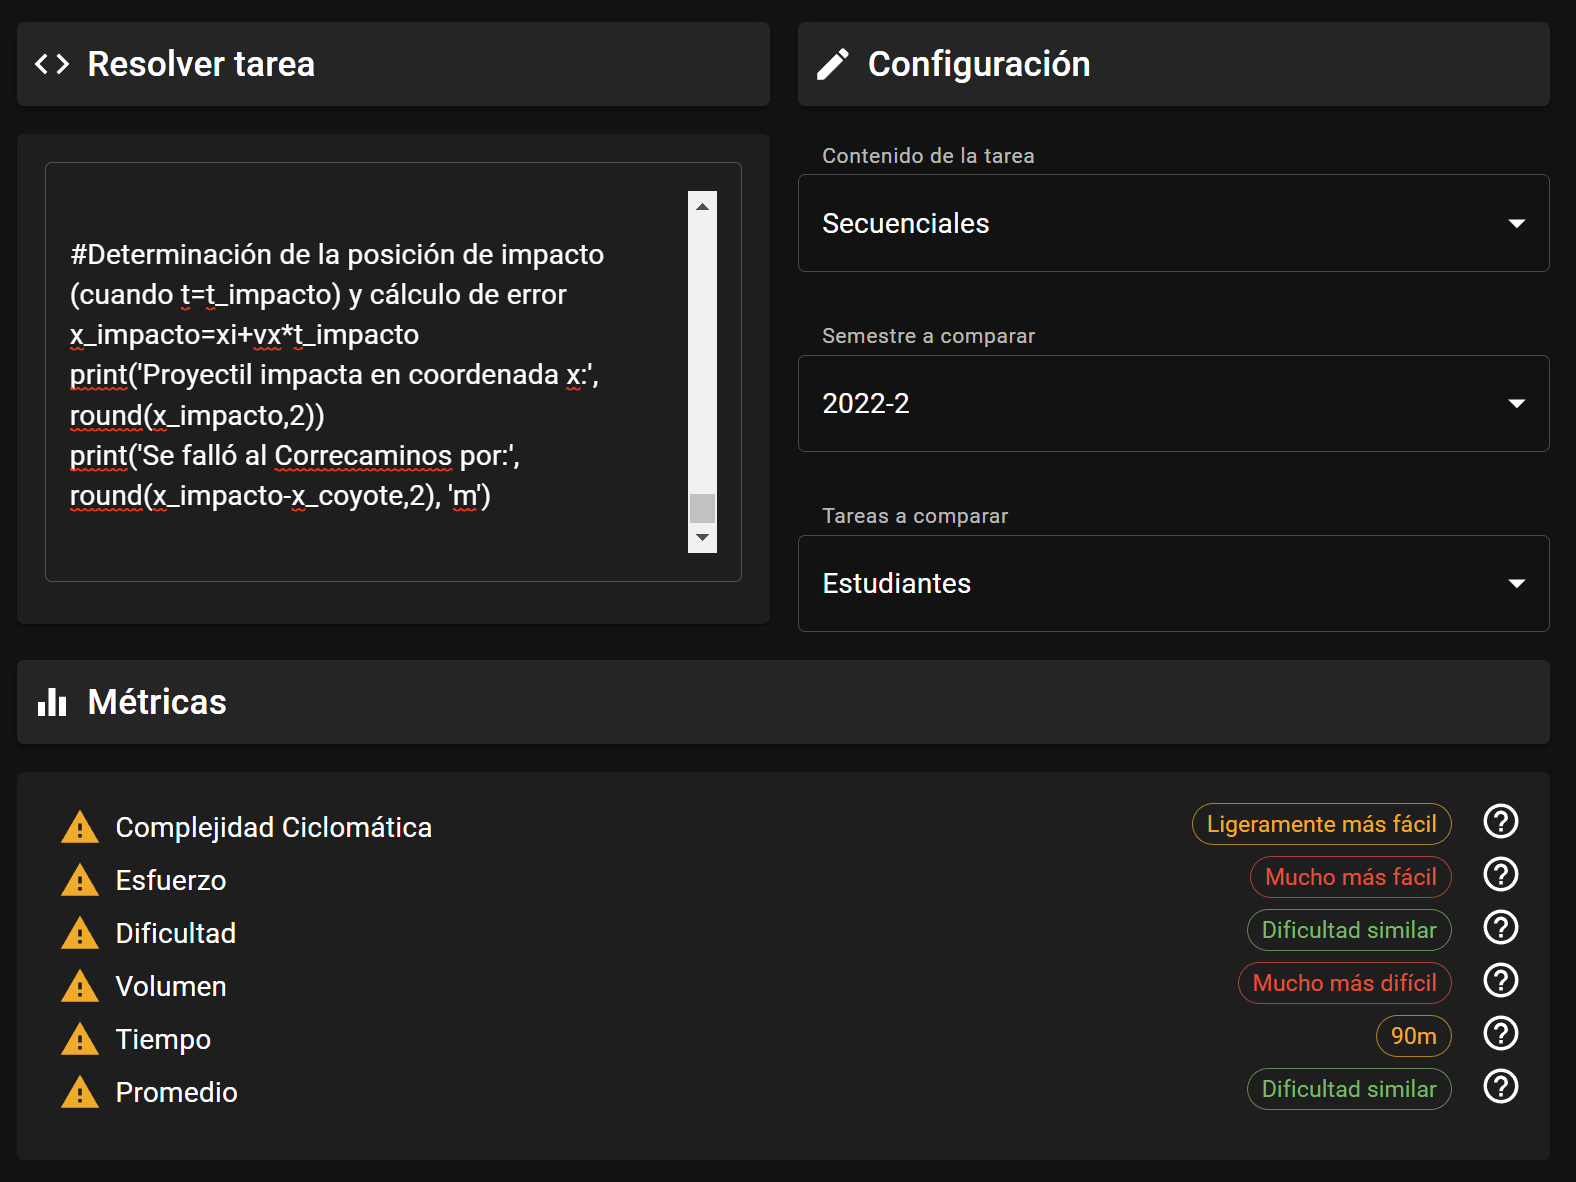
\includegraphics[width=1\textwidth]{figures/ishvel4.png}
          \caption{Métricas de una solución según Ishvel.} Fuente: elaboración propia.
          \label{img:ishvel4}
        \end{figure}
  \item Por último, para iterar sobre el enunciado y poder abordar así las métricas de la tarea que se está elaborando, se muestran en la sección \texttt{Sugerencias} una serie de sugerencias que se pueden aplicar, para mejorar la diferencia de dificultad entre la tarea que se está elaborando y la tarea seleccionada para comparar.

        \begin{figure}[H]
          \centering
          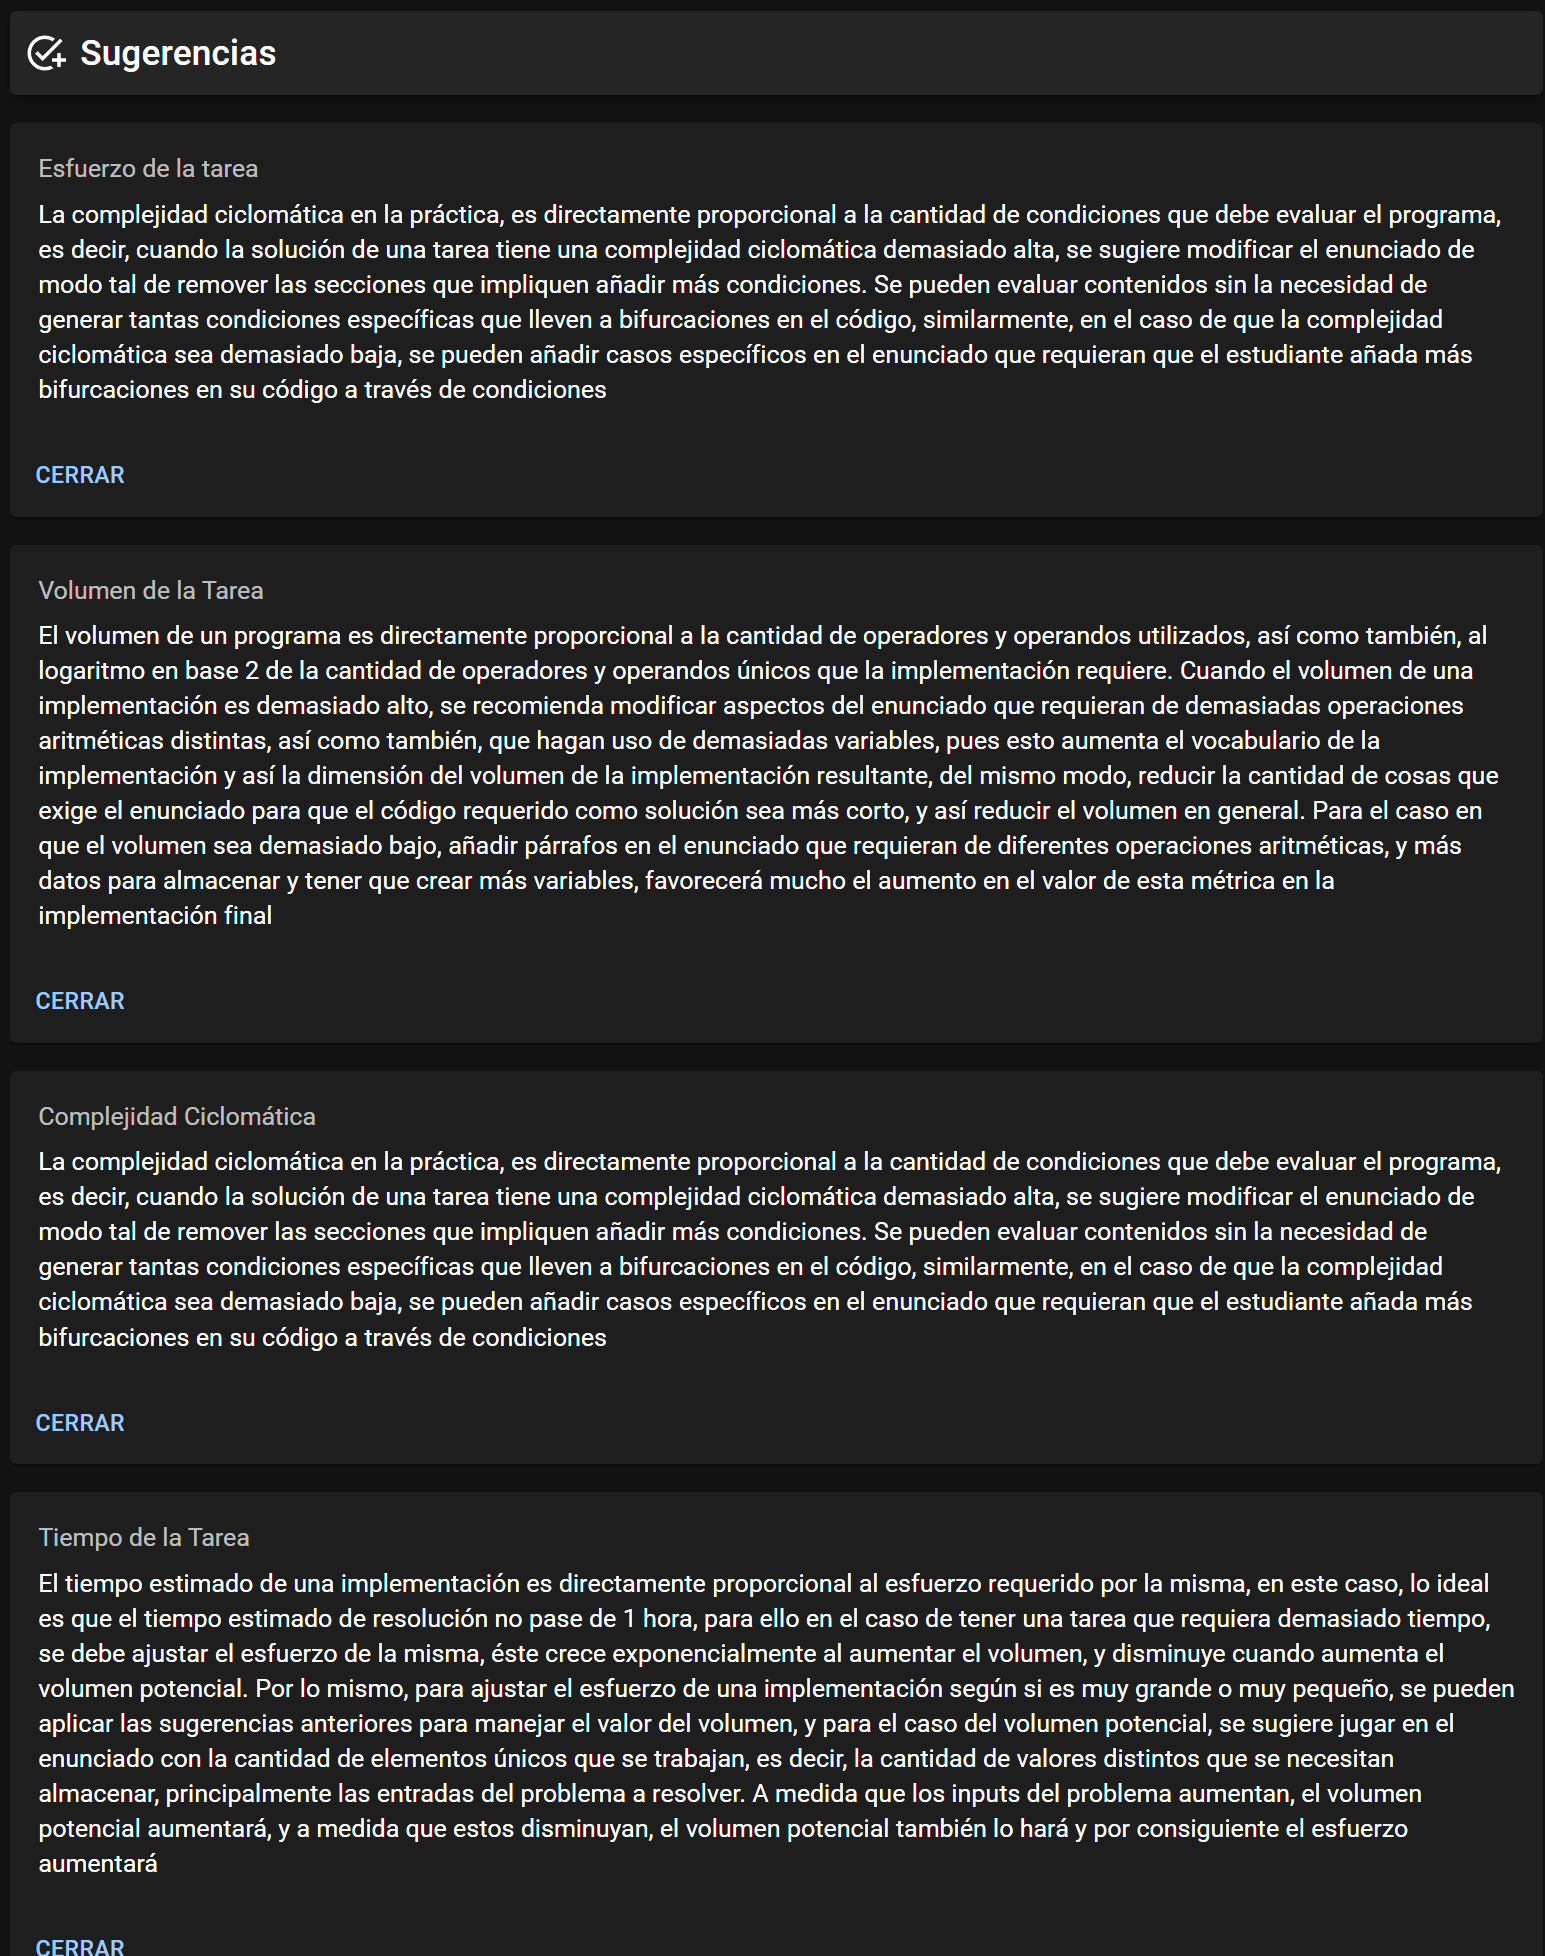
\includegraphics[width=1\textwidth]{figures/ishvel5.png}
          \caption{Sugerencias para una tarea según Ishvel.} Fuente: elaboración propia.
          \label{img:ishvel5}
        \end{figure}
  \item Para descargar la tarea en PDF, se presiona el botón \texttt{Descargar Tarea}
        \begin{figure}[H]
          \centering
          
\includegraphics[width=1\textwidth]{figures/ishvel6.png}
          \caption{Botón de descargar tarea en el editor de Ishvel.} Fuente: elaboración propia.
          \label{img:ishvel6}
        \end{figure}
\end{itemize}

Realizados estos pasos, se puede elaborar una tarea de un curso introductorio de programación teniendo una idea sobre su dificultad antes de publicarla a los estudiantes. Por otro lado, el framework busca también ofrecer métricas históricas para analizar el comportamiento de las tareas en el tiempo, para ésto, se presiona el botón \texttt{Métricas Históricas} al lado del botón \texttt{Descargar Tarea} como se ve en la imagen \ref{img:ishvel6}, lo que desplegará las métricas históricas que el framework tiene cargadas.

\begin{figure}[H]
  \centering
  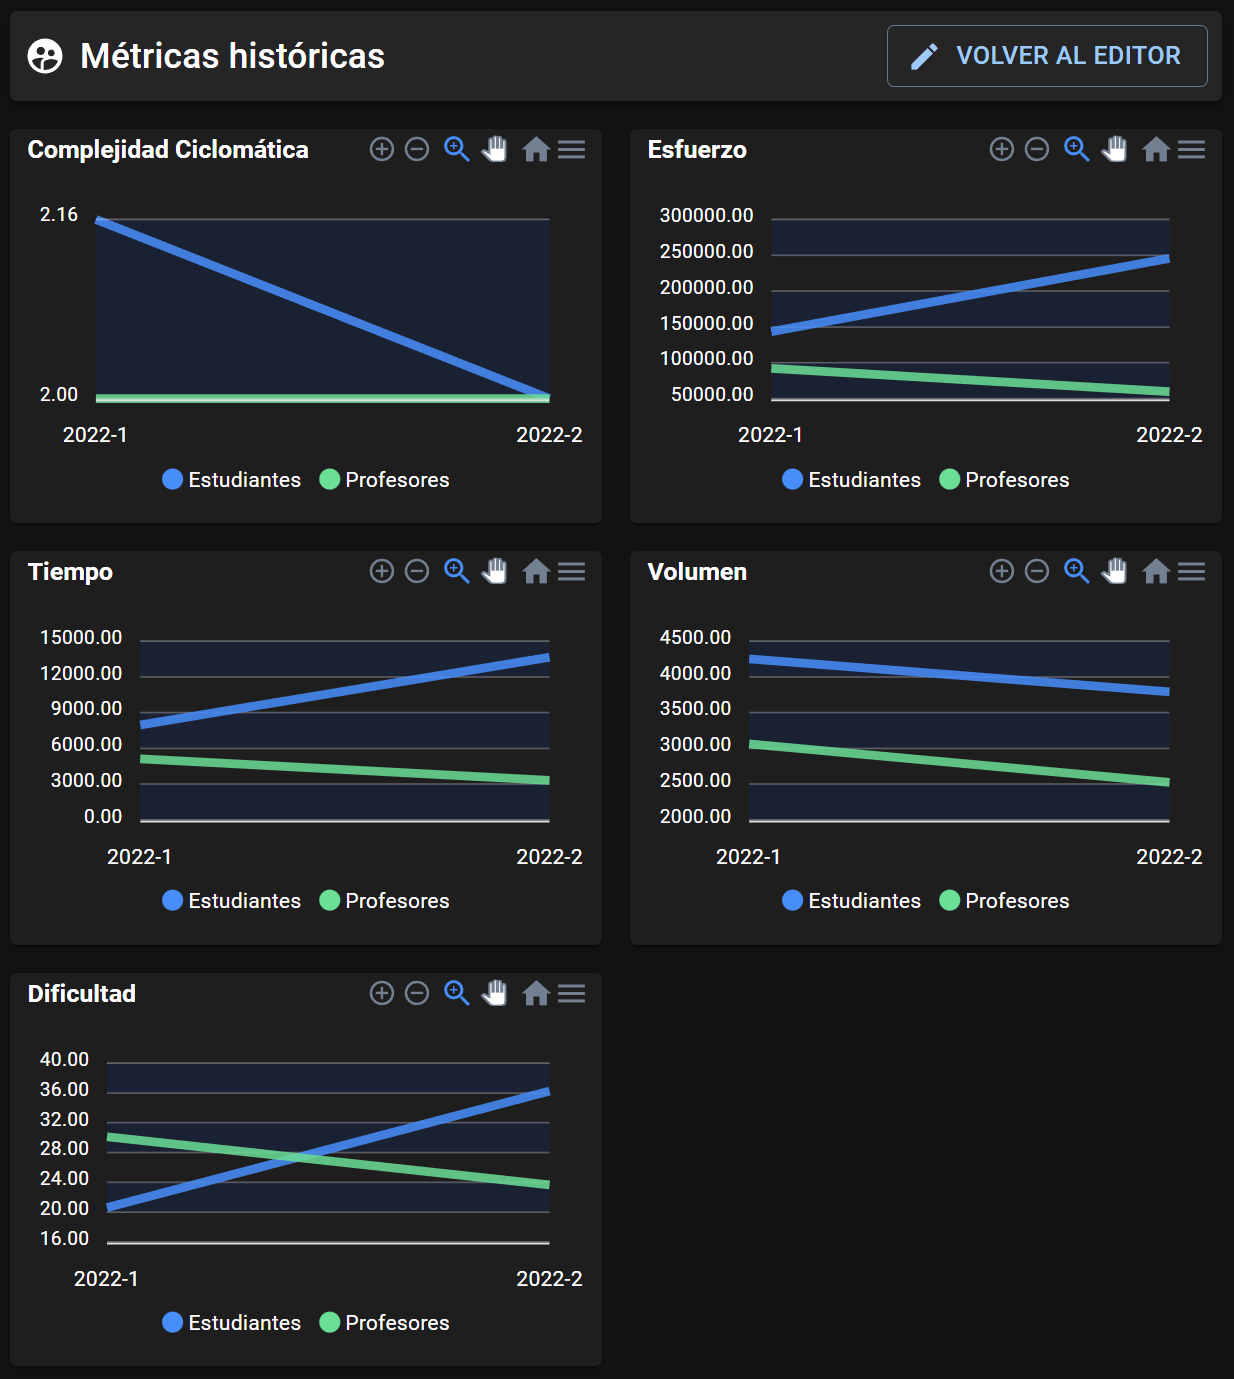
\includegraphics[width=1\textwidth]{figures/ishvel7.png}
  \caption{Sección de métricas históricas del framework Ishvel.} Fuente: elaboración propia.
  \label{img:ishvel7}
\end{figure}

\subsubsection{Cálculo de Métricas} \label{sssec:metricsCalc}

El framework trae consigo una herramienta llamada \textit{metrics-research}, la cual hace uso del módulo multimetricprog \cite{privkweihmann_multimetricprog} para calcular de manera programática las métricas de tanto 1 solución, como el promedio de métricas de varias soluciones al mismo tiempo.

Para utilizar la herramienta, se debe navegar en una terminal hasta el directorio que la contiene, y luego ejecutar el programa \texttt{main.py} que se encuentra en utilizando alguno de los siguientes parámetros:

\begin{itemize}
  \item \textbf{-f FILE}: Indica en FILE la ruta del archivo cuyas métricas se desean calcular.
        \begin{figure}[H]
          \centering
          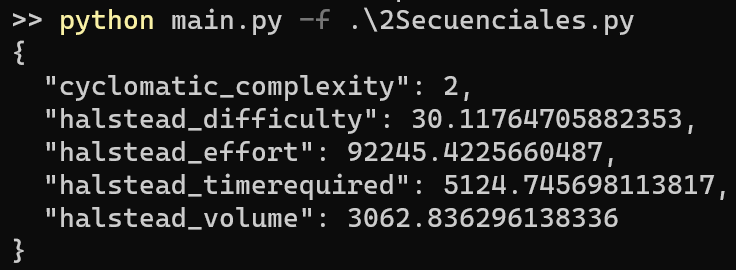
\includegraphics[width=1\textwidth]{figures/metricstool1.png}
          \caption{Ejemplo de uso de la herramienta metrics-research con el parámetro -f.} Fuente: elaboración propia.
          \label{metricstool1}
        \end{figure}
  \item \textbf{-d DIR}: Indica en DIR el directorio de la carpeta con las soluciones cuyo promedio de métricas se desea calcular.
        \begin{figure}[H]
          \centering
          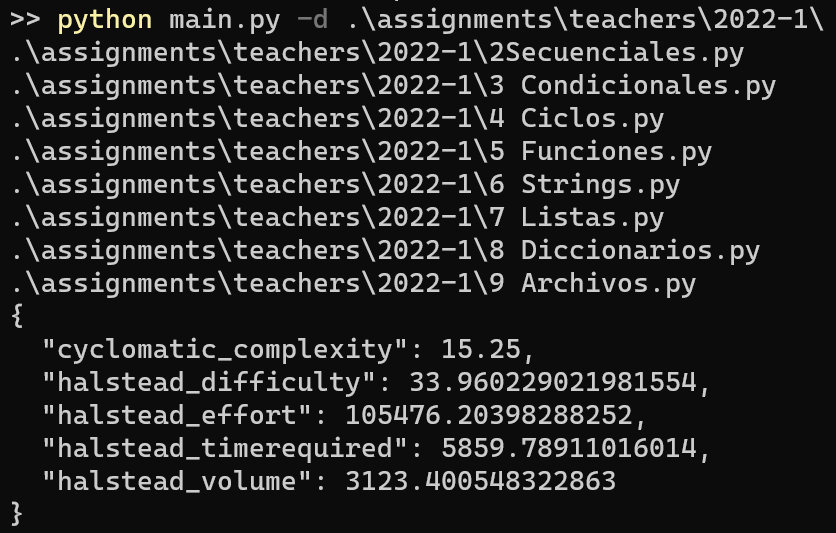
\includegraphics[width=0.8\textwidth]{figures/metricstool2.png}
          \caption{Ejemplo de uso de la herramienta metrics-research con el parámetro -d.} Fuente: elaboración propia.
          \label{metricstool2}
        \end{figure}
  \item \textbf{-h}: Se consulta la documentación de los parámetros del programa.
        \begin{figure}[H]
          \centering
          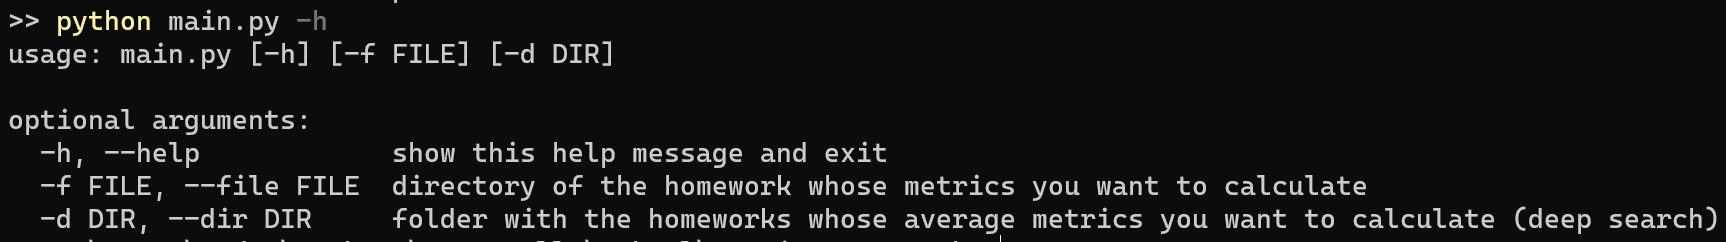
\includegraphics[width=1\textwidth]{figures/metricstool3.png}
          \caption{Ejemplo de uso de la herramienta metrics-research con el parámetro -h.} Fuente: elaboración propia.
          \label{metricstool3}
        \end{figure}
\end{itemize}

\subsubsection{Determinar la Diferencia de Dificultad entre Tareas}

La diferencia de dificultad entre tareas, se calcula utilizando el promedio de los intervalos a los que pertenezca la diferencia porcentual de cada métrica, sin considerar la métrica de \textbf{tiempo de resolución}. Para determinar esto, se realiza el siguiente procedimiento para cada métrica entre 2 tareas:
\begin{enumerate}
  \item Se define un conjunto de \textbf{intervalos de comparación de dificultad}, éstos corresponden a 5 intervalos que categorizan la diferencia de dificultad entre 2 tareas, utilizando las diferencias porcentuales de las métricas de las mismas.
  \item Se calcula la diferencia porcentual entre los valores de la métrica con la que se esté trabajando de ambas tareas.
  \item Se determina el intervalo de comparación de dificultad al que pertenece la diferencia porcentual calculada
\end{enumerate}
Una vez que se obtiene el intervalo de comparación de dificultad al que pertenecen cada una de las métricas de ambas tareas, se promedian los resultados y se redondea al entero más cercano. El valor de este resultado indicará la diferencia de dificultad entre ambas tareas, según la siguiente clasificación:
\begin{enumerate}
  \item Mucho más fácil
  \item Más fácil
  \item Similar
  \item Más difícil
  \item Mucho más difícil
\end{enumerate}
Para entender mejor esta parte de la metodología, se presenta el siguiente ejemplo:

Sean los intervalos de comparación de dificultad para las métricas consideradas:

\begin{table}[H]
  \centering
  \begin{tabular}{|l|r|r|r|r|}
    \hline
    \textbf{Intervalo}    & \multicolumn{1}{l|}{\textbf{Complejidad Ciclomática}} & \multicolumn{1}{l|}{\textbf{Dificultad H.}} & \multicolumn{1}{l|}{\textbf{Esfuerzo}} & \multicolumn{1}{l|}{\textbf{Volumen}} \\ \hline
    1 - mucho más fácil   & -inf\%, -50\%                                         & -inf\%, -25\%                               & -inf\%, -75\%                          & -inf\%, -35\%                         \\ \hline
    2 - más fácil         & -49\%, -5\%                                           & -24\%, -15\%                                & -74\%, -25\%                           & -34\%, 5\%                            \\ \hline
    3 - similar           & -4\%, 25\%                                            & -14\%, 5\%                                  & -24\%, 15\%                            & 6\%, 30\%                             \\ \hline
    4 - más difícil       & 26\%, 70\%                                            & 6\%, 50\%                                   & 16\%, 65\%                             & 31\%, 55\%                            \\ \hline
    5 - mucho más difícil & 71\%, inf\%                                           & 51\%, inf\%                                 & 66\%, inf\%                            & 56\%, inf\%                           \\ \hline
  \end{tabular}
  \caption{Ejemplo de intervalos de comparación de dificultad para todas las métricas, a excepción del tiempo estimado.} Fuente: elaboración propia
  \label{tab:example-difficulty-interval}
\end{table}

Y las métricas de 2 tareas del mismo contenido, junto con sus respectivas diferencias porcentuales:

\begin{table}[H]
  \centering
  \begin{tabular}{l|r|r|r|r|}
    \cline{2-5}
                                                         & \multicolumn{1}{l|}{\textbf{Complejidad Ciclomática}} & \multicolumn{1}{l|}{\textbf{Dificultad H.}} & \multicolumn{1}{l|}{\textbf{Esfuerzo}} & \multicolumn{1}{l|}{\textbf{Volumen}} \\ \cline{2-5}
                                                         & 16                                                    & 30                                          & 2255                                   & 730                                   \\ \cline{2-5}
                                                         & 17                                                    & 44                                          & 1520                                   & 342                                   \\ \hline
    \multicolumn{1}{|l|}{\textbf{Diferencia Porcentual}} & 6.25\%                                                & 46.66\%                                     & -32.59\%                               & -53.15                                \\ \hline
  \end{tabular}
  \caption{Ejemplo de métricas de dos tareas del mismo contenido.} Fuente: elaboración propia
  \label{tab:example-metrics-two-homeworks}
\end{table}

Se determina a qué intervalo pertenece la diferencia porcentual de cada una de las métricas, obteniendo los siguientes valores:

\begin{itemize}
  \item Complejidad Ciclomática: \textbf{3 - similar}
  \item Dificultad H.: \textbf{4 - más difícil}
  \item Esfuerzo: \textbf{2 - más fácil}
  \item Volumen: \textbf{1 - mucho más fácil}
\end{itemize}

Finalmente, se calcula la diferencia de dificultad entre ambas tareas como el promedio redondeado de las categorías de las métricas, es decir, 3. Por lo tanto, aplicando la metodología del framework Ishvel, ambas tareas tienen una dificultad similar, o dicho de otra manera, la resolución de la tarea que se está elaborando, tiene una dificultad similar a la de una tarea desarrollada previamente del mismo contenido.

\subsubsection{Determinar los Intervalos de Comparación de Dificultad entre Tareas}

Los intervalos de comparación de dificultad mencionados anteriormente, son los que se utilizan para poder extraer información sobre la diferencia porcentual de una métrica entre 2 tareas. Para determinarlos, se requiere primero plantear qué dificultades comparativas y métricas se utilizarán en el proceso:

Sean las dificultades comparativas:

\begin{enumerate}
  \item Mucho más fácil
  \item Más fácil
  \item Similar
  \item Más difícil
  \item Mucho más difícil
\end{enumerate}


Y las métricas contempladas para determinar la dificultad entre 2 tareas:

\begin{enumerate}
  \item Complejidad ciclomática
  \item Dificultad según Halstead (Dificultad H.)
  \item Esfuerzo
  \item Volumen
\end{enumerate}

Lo que se busca es definir:

\begin{itemize}
  \item $LI_{dm}$: Límite \textbf{inferior} de la dificultad comparativa $d$ asociado a la métrica $m$, con $d = \left\{1, 2, 3, 4, 5\right\}$ para cada dificultad comparativa respectivamente, y $m = \left\{1, 2, 3, 4\right\}$ para cada métrica, sin contar la métrica de tiempo estimado.
  \item $LS_{dm}$: Límite \textbf{superior} de la dificultad comparativa $d$ asociado a la métrica $m$, con $d = \left\{1, 2, 3, 4, 5\right\}$ para cada dificultad comparativa respectivamente, y $m = \left\{1, 2, 3, 4\right\}$ para cada métrica, sin contar la métrica de tiempo estimado.
\end{itemize}

Para determinar los intervalos de comparación de dificultad, se requiere de una evaluación por un conjunto de expertos en programación, éstos pueden ser docentes, ayudantes docentes y personas con experiencia en el área de la informática. Una vez se cuenta con el conjunto de expertos, se les debe entregar 2 tareas que evalúen contenidos similares, pero que fueron desarrolladas durante periodos lectivos distintos. El panel de expertos tomará ambas tareas, y evaluará según su juicio la dificultad de una tarea en comparación con la otra, siendo las posibles respuestas:

\begin{enumerate}
  \item La segunda tarea es mucho más fácil que la primera tarea
  \item La segunda tarea es más fácil que la primera tarea
  \item La segunda tarea tiene una dificultad similar a la primera tarea
  \item La segunda tarea es más difícil que la primera tarea
  \item La segunda tarea es mucho más difícil que la primera tarea
\end{enumerate}

Una vez obtenidas las respuestas del conjunto de expertos, se debe calcular la diferencia porcentual entre cada una de las métricas de ambas tareas, sin considerar la métrica de tiempo estimado, puesto que ésta es directamente proporcional a la métrica de esfuerzo. Se debe repetir el proceso con varias tareas para obtener la mayor información posible, especialmente con tareas cuya dificultad en comparación sea distinta a la de las otras tareas ya evaluadas. El objetivo de obtener esta información, es relacionar las diferencias porcentuales con los niveles de diferencias de dificultad entre tareas, de manera de tener para cada métrica distintos intervalos de diferencias porcentuales, entre los cuales determinar la dificultad de una tarea en comparación con otra.

A continuación se muestra un ejemplo de la información resultante al término de este paso:

\begin{table}[H]
  \centering
  \begin{tabular}{|l|l|r|r|r|r|}
    \hline
    \textbf{Tareas} & \textbf{\begin{tabular}[c]{@{}l@{}}Comparación de \\ dificultad \end{tabular}} & \multicolumn{1}{l|}{\textbf{\begin{tabular}[c]{@{}l@{}}Complejidad \\ ciclomática (dif \%)\end{tabular}}} & \multicolumn{1}{l|}{\textbf{\begin{tabular}[c]{@{}l@{}}Dificultad H.\\ (dif \%)\end{tabular}}} & \multicolumn{1}{l|}{\textbf{\begin{tabular}[c]{@{}l@{}}Esfuerzo\\ (dif \%)\end{tabular}}} & \multicolumn{1}{l|}{\textbf{\begin{tabular}[c]{@{}l@{}}Volumen\\ (dif \%)\end{tabular}}} \\ \hline
    1 - 2           & 1 - mucho más fácil                                                            & 6,25\%                                                                                                    & 43,69\%                                                                                        & -32,61\%                                                                                  & -32,61\%                                                                                 \\ \hline
    3 - 4           & 2 - más fácil                                                                  & -37,50\%                                                                                                  & -2,86\%                                                                                        & -32,65\%                                                                                  & -32,65\%                                                                                 \\ \hline
    5 - 6           & 3 - similar                                                                    & -18,75\%                                                                                                  & -54,06\%                                                                                       & -76,65\%                                                                                  & -76,65\%                                                                                 \\ \hline
    7 - 8           & 1 - mucho más fácil                                                            & 0,00\%                                                                                                    & -21,46\%                                                                                       & -35,27\%                                                                                  & -35,27\%                                                                                 \\ \hline
    9 - 10          & 5 - mucho más difícil                                                          & 54,55\%                                                                                                   & 66,39\%                                                                                        & 250,00\%                                                                                  & 515,61\%                                                                                 \\ \hline
    11 - 12         & 1 - mucho más fácil                                                            & 50,00\%                                                                                                   & 79,59\%                                                                                        & -2,34\%                                                                                   & -2,34\%                                                                                  \\ \hline
    13 - 14         & 2 - más fácil                                                                  & 40,00\%                                                                                                   & 0,00\%                                                                                         & -15,12\%                                                                                  & -15,12\%                                                                                 \\ \hline
    15 - 16         & 3 - similar                                                                    & 26,32\%                                                                                                   & 54,55\%                                                                                        & 3,46\%                                                                                    & 3,46\%                                                                                   \\ \hline
    17 - 18         & 1 - mucho más fácil                                                            & 43,69\%                                                                                                   & 50,00\%                                                                                        & -32,61\%                                                                                  & 66,39\%                                                                                  \\ \hline
    19 - 20         & 5 - mucho más difícil                                                          & -2,86\%                                                                                                   & 40,00\%                                                                                        & -32,65\%                                                                                  & 79,59\%                                                                                  \\ \hline
    21 - 22         & 1 - mucho más fácil                                                            & -54,06\%                                                                                                  & 26,32\%                                                                                        & -76,65\%                                                                                  & 0,00\%                                                                                   \\ \hline
    23 - 24         & 2 - más fácil                                                                  & -21,46\%                                                                                                  & 43,69\%                                                                                        & -35,27\%                                                                                  & 54,55\%                                                                                  \\ \hline
    25 - 26         & 3 - similar                                                                    & 66,39\%                                                                                                   & -2,86\%                                                                                        & 515,61\%                                                                                  & 50,00\%                                                                                  \\ \hline
    27 - 28         & 1 - mucho más fácil                                                            & 79,59\%                                                                                                   & -54,06\%                                                                                       & -2,34\%                                                                                   & 40,00\%                                                                                  \\ \hline
    29 - 30         & 5 - mucho más difícil                                                          & 3,87\%                                                                                                    & -21,46\%                                                                                       & -15,12\%                                                                                  & 26,32\%                                                                                  \\ \hline
  \end{tabular}
  \caption{Ejemplo de la comparación de dificultad entre tareas, junto con las diferencias porcentuales de cada una de sus métricas.} Fuente: elaboración propia
  \label{tab:example-tasks-comparision}
\end{table}

Ahora, lo que se busca es determinar 5 intervalos de diferencias porcentuales para cada métrica, donde cada intervalo corresponde a una de las 5 dificultades comparativas posibles, para así poder comparar las métricas de distintas tareas entre sí. Para ésto, se debe seguir el siguiente procedimiento para cada una de las métricas:

\begin{enumerate}
  \item Se crea una tabla con 5 filas y 5 columnas, donde las filas corresponden a los intervalos de las dificultades comparativas, y las columnas corresponden a las métricas asociadas a cada intervalo.
        \begin{table}[H]
          \centering
          \begin{tabular}{|l|l|l|l|l|}
            \hline
            Comparación de Dificultad              & Complejidad Ciclomática & Dificultad H. & Esfuerzo  & Volumen   \\ \hline
            \multirow{2}{*}{1 - mucho más fácil}   & $LI_{11}$               & $LI_{12}$     & $LI_{13}$ & $LI_{14}$ \\ \cline{2-5}
                                                   & $LS_{11}$               & $LS_{12}$     & $LS_{13}$ & $LS_{14}$ \\ \hline
            \multirow{2}{*}{2 - más fácil}         & $LI_{21}$               & $LI_{22}$     & $LI_{23}$ & $LI_{24}$ \\ \cline{2-5}
                                                   & $LS_{21}$               & $LS_{22}$     & $LS_{23}$ & $LS_{24}$ \\ \hline
            \multirow{2}{*}{3 - similar}           & $LI_{31}$               & $LI_{32}$     & $LI_{33}$ & $LI_{34}$ \\ \cline{2-5}
                                                   & $LS_{31}$               & $LS_{32}$     & $LS_{33}$ & $LS_{34}$ \\ \hline
            \multirow{2}{*}{4 - más difícil}       & $LI_{41}$               & $LI_{42}$     & $LI_{43}$ & $LI_{44}$ \\ \cline{2-5}
                                                   & $LS_{41}$               & $LS_{42}$     & $LS_{43}$ & $LS_{44}$ \\ \hline
            \multirow{2}{*}{5 - mucho más difícil} & $LI_{51}$               & $LI_{52}$     & $LI_{53}$ & $LI_{54}$ \\ \cline{2-5}
                                                   & $LS_{51}$               & $LS_{52}$     & $LS_{53}$ & $LS_{54}$ \\ \hline
          \end{tabular}
          \caption{Tabla base de intervalos por métrica para cada dificultad comparativa.} Fuente: elaboración propia
          \label{tab:base-int-table}
        \end{table}

  \item En el primer y último intervalo de la métrica, colocar -inf\% e inf\% respectivamente.
        \begin{table}[H]
          \centering
          \begin{tabular}{|l|l|l|l|l|}
            \hline
            Comparación de Dificultad              & Complejidad Ciclomática & Dificultad H. & Esfuerzo & Volumen \\ \hline
            \multirow{2}{*}{1 - mucho más fácil}   & -inf\%                  &               &          &         \\ \cline{2-5}
                                                   &                         &               &          &         \\ \hline
            \multirow{2}{*}{2 - más fácil}         &                         &               &          &         \\ \cline{2-5}
                                                   &                         &               &          &         \\ \hline
            \multirow{2}{*}{3 - similar}           &                         &               &          &         \\ \cline{2-5}
                                                   &                         &               &          &         \\ \hline
            \multirow{2}{*}{4 - más difícil}       &                         &               &          &         \\ \cline{2-5}
                                                   &                         &               &          &         \\ \hline
            \multirow{2}{*}{5 - mucho más difícil} &                         &               &          &         \\ \cline{2-5}
                                                   & inf\%                   &               &          &         \\ \hline
          \end{tabular}
          \caption{Tabla base de intervalos por métrica para cada dificultad comparativa con los límites máximos y mínimos del primer y último intervalo listos.} Fuente: elaboración propia
          \label{tab:base-int-table-infs}
        \end{table}
  \item A partir del intervalo de la primera dificultad comparativa ``mucho más fácil'', se calcula el límite superior restante como el mínimo entre la máxima diferencia porcentual de esa dificultad comparativa, y la mínima diferencia porcentual de la dificultad comparativa siguiente, en este caso -37.50\%.

        \begin{table}[H]
          \centering
          \begin{tabular}{|l|l|l|l|l|}
            \hline
            \textbf{Comparación de Dificultad}     & \textbf{Complejidad Ciclomática} & \textbf{Dificultad H.} & \textbf{Esfuerzo} & \textbf{Volumen} \\ \hline
            \multirow{2}{*}{1 - mucho más fácil}   & -inf\%                           & -inf\%                 & -inf\%            & -inf\%           \\ \cline{2-5}
                                                   & \multicolumn{1}{r|}{-37,50\%}    &                        &                   &                  \\ \hline
            \multirow{2}{*}{2 - más fácil}         & \multicolumn{1}{r|}{}            &                        &                   &                  \\ \cline{2-5}
                                                   & \multicolumn{1}{r|}{}            &                        &                   &                  \\ \hline
            \multirow{2}{*}{3 - similar}           & \multicolumn{1}{r|}{}            &                        &                   &                  \\ \cline{2-5}
                                                   & \multicolumn{1}{r|}{}            &                        &                   &                  \\ \hline
            \multirow{2}{*}{4 - más difícil}       &                                  &                        &                   &                  \\ \cline{2-5}
                                                   &                                  &                        &                   &                  \\ \hline
            \multirow{2}{*}{5 - mucho más difícil} &                                  &                        &                   &                  \\ \cline{2-5}
                                                   & inf\%                            & inf\%                  & inf\%             & inf\%            \\ \hline
          \end{tabular}
          \caption{Tabla base de intervalos por métrica para cada dificultad comparativa con el primer intervalo listo.} Fuente: elaboración propia
          \label{tab:base-int-table-1}
        \end{table}
  \item Se continúa con el intervalo de la siguiente dificultad comparativa, donde su límite inferior se calcula como el límite superior anterior + 0.01\%, lo que en este caso resulta en -37.49\%.
        \begin{table}[H]
          \centering
          \begin{tabular}{|l|l|l|l|l|}
            \hline
            \textbf{Comparación de Dificultad}     & \textbf{Complejidad Ciclomática} & \textbf{Dificultad H.} & \textbf{Esfuerzo} & \textbf{Volumen} \\ \hline
            \multirow{2}{*}{1 - mucho más fácil}   & -inf\%                           & -inf\%                 & -inf\%            & -inf\%           \\ \cline{2-5}
                                                   & \multicolumn{1}{r|}{-37,50\%}    &                        &                   &                  \\ \hline
            \multirow{2}{*}{2 - más fácil}         & \multicolumn{1}{r|}{-37,49\%}    &                        &                   &                  \\ \cline{2-5}
                                                   & \multicolumn{1}{r|}{}            &                        &                   &                  \\ \hline
            \multirow{2}{*}{3 - similar}           & \multicolumn{1}{r|}{}            &                        &                   &                  \\ \cline{2-5}
                                                   & \multicolumn{1}{r|}{}            &                        &                   &                  \\ \hline
            \multirow{2}{*}{4 - más difícil}       &                                  &                        &                   &                  \\ \cline{2-5}
                                                   &                                  &                        &                   &                  \\ \hline
            \multirow{2}{*}{5 - mucho más difícil} &                                  &                        &                   &                  \\ \cline{2-5}
                                                   & inf\%                            & inf\%                  & inf\%             & inf\%            \\ \hline
          \end{tabular}
          \caption{Tabla base de intervalos por métrica para cada dificultad comparativa con el límite inferior del segundo intervalo.} Fuente: elaboración propia
          \label{tab:base-int-table-2}
        \end{table}
  \item Se repiten los pasos 3 y 4 hacia los intervalos posteriores.
        \begin{table}[H]
          \centering
          \begin{tabular}{|l|l|l|l|l|}
            \hline
            \textbf{Comparación de Dificultad}     & \textbf{Complejidad Ciclomática} & \textbf{Dificultad H.} & \textbf{Esfuerzo} & \textbf{Volumen} \\ \hline
            \multirow{2}{*}{1 - mucho más fácil}   & -inf\%                           & -inf\%                 & -inf\%            & -inf\%           \\ \cline{2-5}
                                                   & \multicolumn{1}{r|}{-37,50\%}    &                        &                   &                  \\ \hline
            \multirow{2}{*}{2 - más fácil}         & \multicolumn{1}{r|}{-37,49\%}    &                        &                   &                  \\ \cline{2-5}
                                                   & \multicolumn{1}{r|}{-18,75\%}    &                        &                   &                  \\ \hline
            \multirow{2}{*}{3 - similar}           & \multicolumn{1}{r|}{-18,74\%}    &                        &                   &                  \\ \cline{2-5}
                                                   & \multicolumn{1}{r|}{66,39\%}     &                        &                   &                  \\ \hline
            \multirow{2}{*}{4 - más difícil}       &                                  &                        &                   &                  \\ \cline{2-5}
                                                   &                                  &                        &                   &                  \\ \hline
            \multirow{2}{*}{5 - mucho más difícil} &                                  &                        &                   &                  \\ \cline{2-5}
                                                   & inf\%                            & inf\%                  & inf\%             & inf\%            \\ \hline
          \end{tabular}
          \caption{Tabla base de intervalos por métrica para cada dificultad comparativa casi completa para una métrica.} Fuente: elaboración propia
          \label{tab:base-int-table-3}
        \end{table}
  \item En caso de que falte información sobre alguna de las dificultades comparativas, posiblemente porque de la muestra de tareas para el conjunto de expertos, ningún par de tareas fue considerado dentro de alguna dificultad comparativa específica, se debe seguir el siguiente procedimiento:
        \begin{itemize}
          \item Si falta información para la dificultad comparativa 1:
                \begin{itemize}
                  \item Se utiliza el límite inferior de la dificultad comparativa 2 menos 0.01\%, es decir: $LI_{2m} - 0.01\%$, como límite superior. Si no está definido $LI_{2m}$, se considera la menor diferencia porcentual de la dificultad comparativa 2 menos 0.01\% como límite superior.
                \end{itemize}
          \item Si falta información para la dificultad comparativa 2:
                \begin{itemize}
                  \item Se calcula el límite inferior como el límite superior de la dificultad comparativa 1 más 0.01\%, y el límite superior como el límite superior de la dificultad comparativa 1 más 0.01\%, sumado a la distancia entre el límite inferior y superior de la dificultad comparativa 4, es decir:
                        \begin{equation*}
                          LI_{2m} = LS_{1m} + 0.01\%
                        \end{equation*}
                        \begin{equation*}
                          LS_{2m} = LS_{1m} + 0.01\% + abs(LI_{4m} - LS_{4m})
                        \end{equation*}
                \end{itemize}
          \item Si falta información para la dificultad comparativa 3:
                \begin{itemize}
                  \item Se utiliza el límite superior de la dificultad comparativa 2 más 0.01\%, es decir: $LS_{2m} + 0.01\%$, como límite inferior.
                  \item Se utiliza el límite inferior de la dificultad comparativa 4 menos 0.01\%, es decir: $LI_{4m} - 0.01\%$, como límite superior.
                \end{itemize}
          \item Si falta información para la dificultad comparativa 4:
                \begin{itemize}
                  \item Se calcula el límite inferior como el límite superior de la dificultad comparativa 3 más 0.01\%, y el límite superior como el límite superior de la dificultad comparativa 3 más 0.01\%, sumado a la distancia entre el límite inferior y superior de la dificultad comparativa 2, es decir:
                        \begin{equation*}
                          LI_{4m} = LS_{3m} + 0.01\%
                        \end{equation*}
                        \begin{equation*}
                          LS_{4m} = LS_{3m} + 0.01\% + abs(LI_{2m} - LS_{2m})
                        \end{equation*}

                \end{itemize}
          \item Si falta información para la dificultad comparativa 5:
                \begin{itemize}
                  \item Se utiliza el límite superior de la dificultad comparativa 4 más 0.01\%, es decir: $LS_{4m} + 0.01\%$, como límite inferior. Si no está definido $LS_{4m}$, se considera la mayor diferencia porcentual más 0.01\% cómo límite inferior.
                \end{itemize}
          \item Si ya se definió el límite inferior de la dificultad comparatida $d$, pero no hay información para definir el superior:
                \begin{itemize}
                  \item Se toma 20 como el tamaño del intervalo, es decir, se calcula el límite superior como $LS_{dm} = LI_{dm} + 20$, dado que 20 sería el tamaño del intervalo si todos los intervalos fuesen iguales.
                \end{itemize}
          \item Si no hay información para definiar los límites de la dificultad comparativa $d$, se debe continuar aplicando la heurística al resto de dificultades comparativas, hasta que hayan suficientes límites definidos como para definir los de la dificultad comparativa $d$.
        \end{itemize}
  \item Se aplican los procedimientos del paso 6 para terminar de rellenar la tabla, y con esto entonces se obtiene la tabla de intervalos de comparación de dificultad para la métrica de complejidad ciclomática.
        \begin{table}[H]
          \centering
          \begin{tabular}{|l|r|l|l|l|}
            \hline
            \textbf{Comparación de Dificultad}     & \multicolumn{1}{l|}{\textbf{Complejidad Ciclomática}} & \textbf{Dificultad H.} & \textbf{Esfuerzo} & \textbf{Volumen} \\ \hline
            \multirow{2}{*}{1 - mucho más fácil}   & \multicolumn{1}{l|}{-inf\%}                           & -inf\%                 & -inf\%            & -inf\%           \\ \cline{2-5}
                                                   & -37,50\%                                              &                        &                   &                  \\ \hline
            \multirow{2}{*}{2 - más fácil}         & -37,49\%                                              &                        &                   &                  \\ \cline{2-5}
                                                   & -18,75\%                                              &                        &                   &                  \\ \hline
            \multirow{2}{*}{3 - similar}           & -18,74\%                                              &                        &                   &                  \\ \cline{2-5}
                                                   & 66,39\%                                               &                        &                   &                  \\ \hline
            \multirow{2}{*}{4 - más difícil}       & 66,40\%                                               &                        &                   &                  \\ \cline{2-5}
                                                   & 85,14\%                                               &                        &                   &                  \\ \hline
            \multirow{2}{*}{5 - mucho más difícil} & 85,15\%                                               &                        &                   &                  \\ \cline{2-5}
                                                   & \multicolumn{1}{l|}{inf\%}                            & inf\%                  & inf\%             & inf\%            \\ \hline
          \end{tabular}
          \caption{Tabla base de intervalos por métrica para cada dificultad comparativa para la métrica de complejidad ciclomática.} Fuente: elaboración propia
          \label{tab:base-int-table-4}
        \end{table}
\end{enumerate}

\subsubsection{Sugerencias}

Dado que el framework da indicios de la dificultad de la tarea en base a su solución, a continuación se presentan estrategias para interpretar cada una de las métricas planteadas en este documento y tomar acciones para ajustarlas:

\begin{itemize}
  \item \textbf{Complejidad ciclomática}: La complejidad ciclomática en la práctica, es directamente proporcional a la cantidad de condiciones que debe evaluar el programa, es decir, cuando la solución de una tarea tiene una complejidad ciclomática demasiado alta, se sugiere modificar el enunciado de modo tal de remover las secciones que impliquen añadir más condiciones. Se pueden evaluar contenidos sin la necesidad de generar tantas condiciones específicas que lleven a bifurcaciones en el código, similarmente, en el caso de que la complejidad ciclomática sea demasiado baja, se pueden añadir casos específicos en el enunciado que requieran que el estudiante añada más bifurcaciones en su código a través de condiciones.
  \item \textbf{Volumen}: El volumen de un programa es directamente proporcional a la cantidad de operadores y operandos utilizados, así como también, al logaritmo en base 2 de la cantidad de operadores y operandos únicos que la implementación requiere. Cuando el volumen de una implementación es demasiado alto, se recomienda modificar aspectos del enunciado que requieran de demasiadas operaciones aritméticas distintas, así como también, que hagan uso de demasiadas variables, pues esto aumenta el vocabulario de la implementación y así la dimensión del volumen de la implementación resultante, del mismo modo, reducir la cantidad de cosas que exige el enunciado para que el código requerido como solución sea más corto, y así reducir el volumen en general. Para el caso en que el volumen sea demasiado bajo, añadir párrafos en el enunciado que requieran de diferentes operaciones aritméticas, y más datos para almacenar y tener que crear más variables, favorecerá mucho el aumento en el valor de esta métrica en la implementación final.
  \item \textbf{Esfuerzo}: El esfuerzo crece exponencialmente al aumentar el volumen, y disminuye cuando aumenta el volumen potencial. Por lo mismo, para ajustar el esfuerzo de una implementación según si es muy grande o muy pequeño, se pueden aplicar las sugerencias anteriores para manejar el valor del volumen, y para el caso del volumen potencial, se sugiere jugar en el enunciado con la cantidad de elementos únicos que se trabajan, es decir, la cantidad de valores distintos que se necesitan almacenar, principalmente las entradas del problema a resolver. A medida que los inputs del problema aumentan, el volumen potencial aumentará, y a medida que estos disminuyan, el volumen potencial también lo hará y por consiguiente el esfuerzo aumentará.
  \item \textbf{Dificultad}: La dificultad de un programa se maneja según el vocabulario $\eta$ y el largo $N$ del mismo. Cuando la cantidad de operadores únicos aumenta, o cuando aumenta el total de operadores únicos utilizados, la dificultad del programa aumenta, mientras que cuando la cantidad de operandos únicos aumenta, la dificultad disminuye. Para ajustar el valor de la dificultad de una implementación según el enunciado de una tarea, sugiere incluír en los párrafos aspectos del enunciado que requieran cálculos con operadores aritméticos variados, o bien, hacer uso de distintos valores a considerar a la hora de realizar el programa, esto puede llevarse a cabo con distintos inputs, o bien, con distintos valores a considerar a la hora de realizar condiciones, poner límites, precios en el caso de programas que requieran tiendas, etc.
  \item \textbf{Tiempo}: El tiempo estimado de una implementación es directamente proporcional al esfuerzo requerido por la misma, en este caso, lo ideal es que el tiempo estimado de resolución no pase de 1 hora, para ello en el caso de tener una tarea que requiera demasiado tiempo, se recomienda aplicar las sugerencias de la métrica de esfuerzo para hacer los ajustes necesarios.
\end{itemize}

\subsubsection{Actualización de Métricas Semestrales} \label{sssec:metricsUpdate}

En el editor del framework, se encuentra en el directorio \texttt{src/core/data} un conjunto de archivos encargados de mantener los datos con los que funciona el software.
\begin{figure}[H]
  \centering
  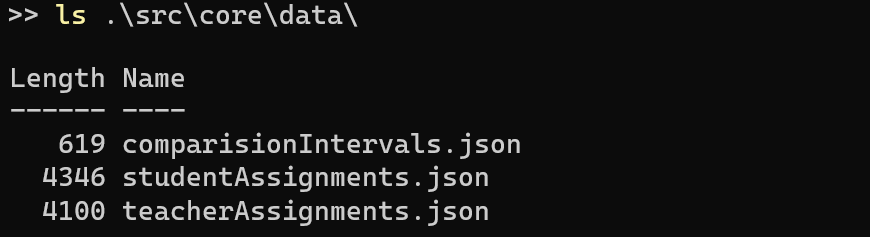
\includegraphics[width=1\textwidth]{figures/datafiles.png}
  \caption{Archivos de datos del editor.} Fuente: elaboración propia.
  \label{datafiles}
\end{figure}
En particular, los archivos \texttt{studentAssignments.json} y \texttt{teacherAssignments.json} contienen respectivamente, las métricas promedio de las soluciones de todos los estudiantes, y las métricas individuales de las soluciones de los profesores a las tareas de los semestres estudiados.

Para actualizar las métricas semestrales, se debe primero calcular el promedio de métricas de las tareas de los estudiantes, así como también las métricas de las soluciones de los profesores a las mismas, siguiendo los pasos de la sección \ref{sssec:metricsCalc}. Luego se deben añadir estos datos al archivo respectivo para que sean desplegadas en las métricas históricas del editor.

Ambos archivos comparten la siguiente estructura:
\begin{figure}[H]
  \centering
  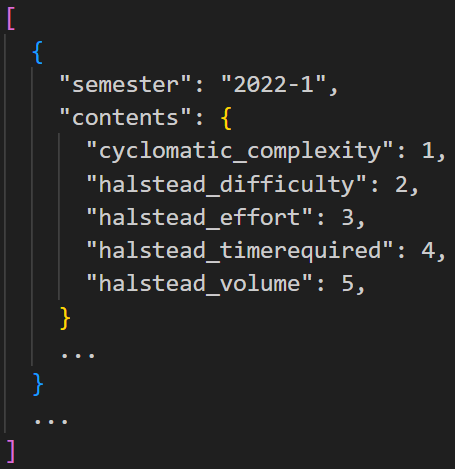
\includegraphics[width=1\textwidth]{figures/metrics1.png}
  \caption{Formato de los archivos de métricas del editor.} Fuente: elaboración propia.
  \label{img:metrics1}
\end{figure}

La cual se compone de una lista de objetos con las siguientes propiedades
\begin{itemize}
  \item \textbf{semester}: Semestre al cual corresponden las métricas
  \item \textbf{content}: Objeto cuyo nombre debe ser el contenido de la tarea, y que sus propiedades serán las métricas de la misma. Para trabajar con los 8 contenidos evaluados en los semestres 2022-1 y 2022-2, se utilizaron como contenidos:
        \begin{itemize}
          \item \textbf{dicts}: Diccionarios
          \item \textbf{files}: Archivos
          \item \textbf{lists}: Listas
          \item \textbf{functions}: Funciones
          \item \textbf{strings}: Strings
          \item \textbf{loops}: Ciclos
          \item \textbf{conditionals}: Condicionales
          \item \textbf{sequential}: Secuenciales
        \end{itemize}
  \item \textbf{cyclomatic\_complexity}: Complejidad ciclomática de la tarea del contenido correspondiente
  \item \textbf{halstead\_difficulty}: Dificultad según Halstead de la tarea del contenido correspondiente
  \item \textbf{halstead\_effort}: Esfuerzo de la tarea del contenido correspondiente
  \item \textbf{halstead\_timerequired}: Tiempo estimado requerido para desarrolllar la tarea del contenido correspondiente
  \item \textbf{halstead\_volume}: Volumen de la tarea del contenido correspondiente
\end{itemize}
Para añadir las métricas de una nueva tarea, ya sea el promedio de las tareas de los estudiantes, o de la solución de los profesores, se debe añadir una nueva llave debajo de las métricas de la última tarea del semestre en curso, esta llave debe tener el nombre del contenido cuyas métricas fueron calculadas, y dentro de esta llave, debe pegarse el resultado de las métricas calculadas con la herramienta \textit{metrics-research}.
\begin{figure}[H]
  \centering
  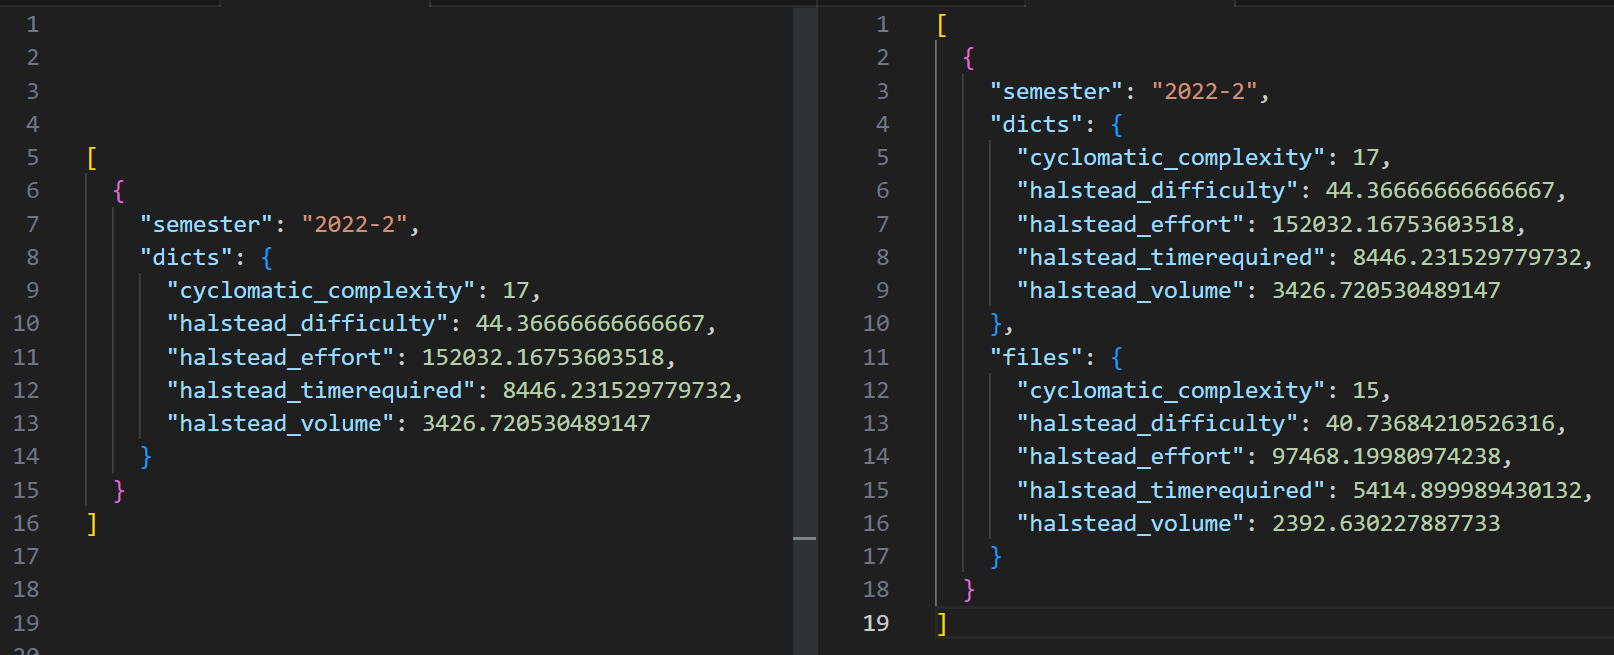
\includegraphics[width=1\textwidth]{figures/metrics2.png}
  \caption{Ejemplo de como añadir las métricas de la tarea de archivos del semestre 2022-2 en el archivo de métricas del editor.} Fuente: elaboración propia.
  \label{img:metrics2}
\end{figure}
En el caso de necesitar añadir un nuevo semestre, se debe añadir un objeto nuevo a la lista, el cual siga el formato de la figura \ref{img:metrics1}, y entonces añadir allí las métricas según el contenido del que se disponga información
\begin{figure}[H]
  \centering
  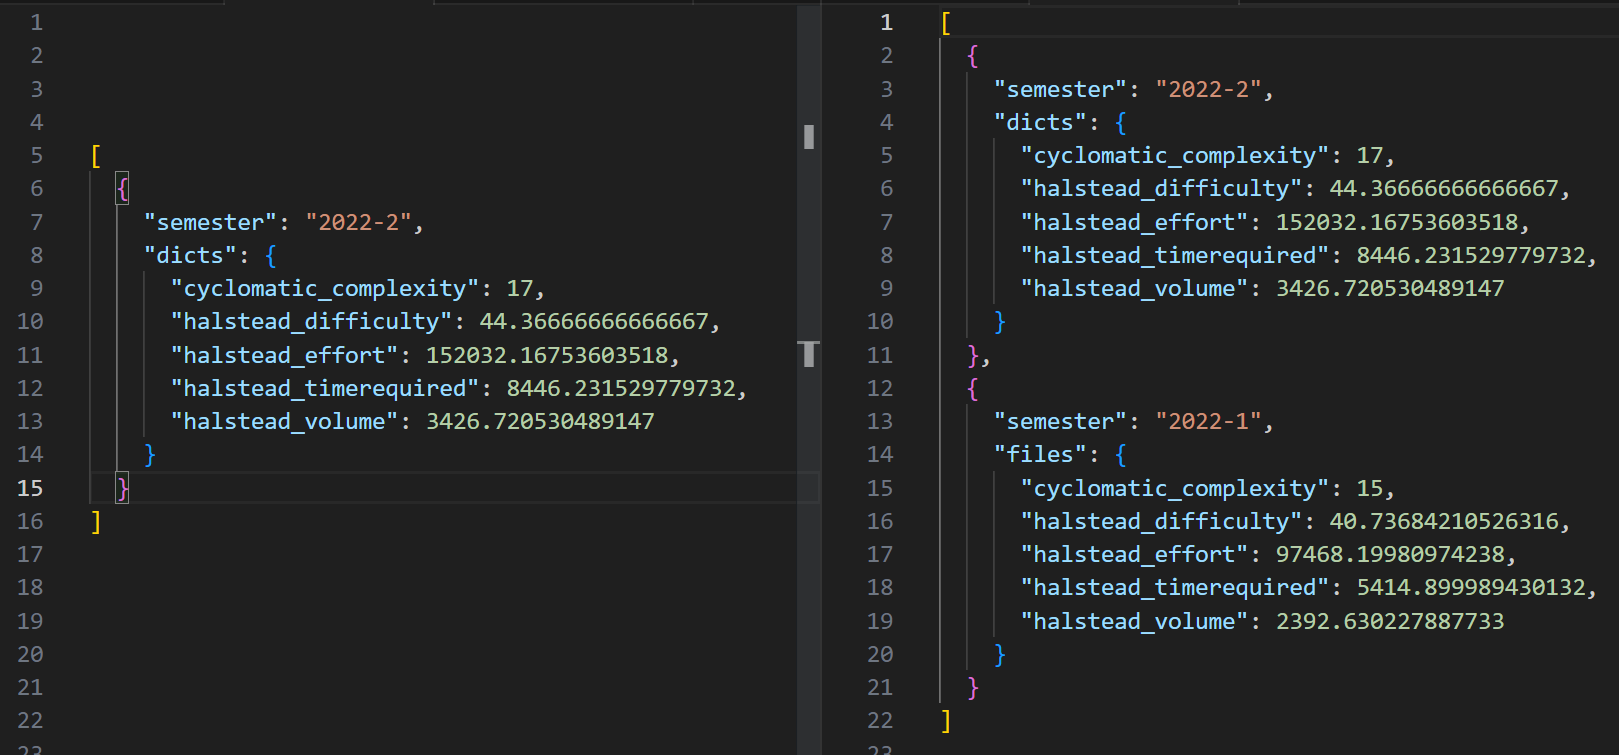
\includegraphics[width=1\textwidth]{figures/metrics3.png}
  \caption{Ejemplo de como añadir las métricas de la tarea de archivos del semestre 2022-3 en el archivo de métricas del editor.} Fuente: elaboración propia.
  \label{img:metrics3}
\end{figure}
\subsubsection{Actualización de Intervalos de Comparación de Dificultad} \label{sssec:comparisionIntMod}

En el editor del framework se encuentra el directorio \texttt{src/core/data}, el cual contiene el archivo \texttt{comparisionIntervals.json} con el siguiente contenido:
\begin{figure}[H]
  \centering
  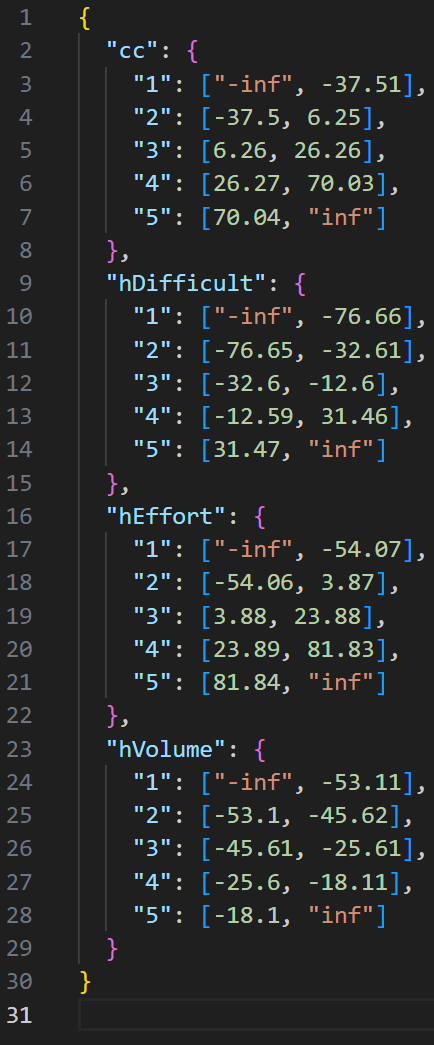
\includegraphics[width=0.5\textwidth]{figures/metrics4.png}
  \caption{Contenido del archivo de intervalos de comparación de dificultad.} Fuente: elaboración propia.
  \label{img:metrics4}
\end{figure}
Cuya estructura consta de:
\begin{itemize}
  \item \textbf{Métrica}: El nombre de la métrica que contendrá los intervalos de comparación de dificultad.
        \begin{itemize}
          \item \textbf{``1''}: Lista con el límite inferior y superior del ntervalo de comparación para la dificultad ``mucho más fácil''.
          \item \textbf{``2''}: Lista con el límite inferior y superior del ntervalo de comparación para la dificultad ``más fácil''.
          \item \textbf{``3''}: Lista con el límite inferior y superior del ntervalo de comparación para la dificultad ``similar''.
          \item \textbf{``4''}: Lista con el límite inferior y superior del ntervalo de comparación para la dificultad ``mucho difícil''.
          \item \textbf{``5''}: Lista con el límite inferior y superior del ntervalo de comparación para la dificultad ``mucho más difícil''.
        \end{itemize}
\end{itemize}
Siendo los nombres de métricas válidas:
\begin{itemize}
  \item \textbf{cc}: Complejidad ciclomática.
  \item \textbf{hDifficult}: Dificultad según Halstead.
  \item \textbf{hEffort}: Esfuerzo.
  \item \textbf{hVolume}: Volumen
\end{itemize}
Para modificar los intervalos de comparación de dificultad, basta con modificar los valores de los límites superiores e inferiores de las métricas.

\subsubsection{Análisis de Métricas entre Semestres}

Para analizar cómo han ido variando las métricas a los largo de los semestres, el framework cuenta con la sección \texttt{Métricas Históricas}, donde se pueden ver gráficos que comparan las métricas de complejidad ciclomática, dificultad, tiempo, esfuerzo y volumen a lo largo de los semestres.
\begin{figure}[H]
  \centering
  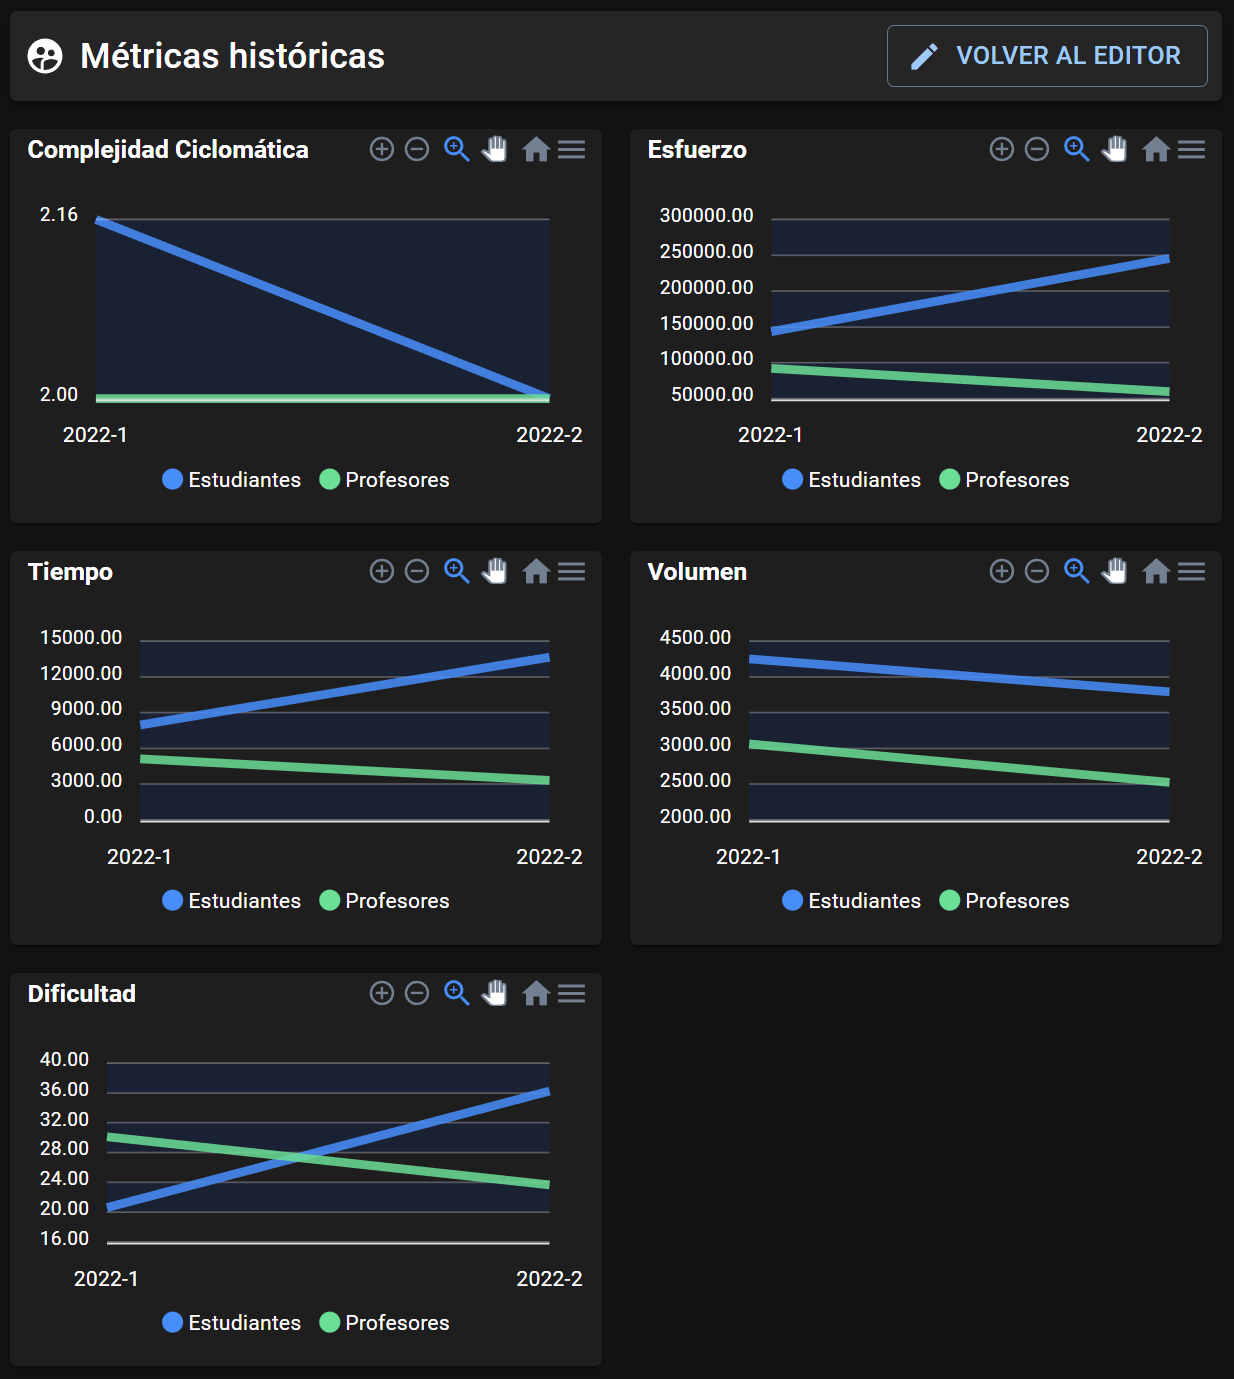
\includegraphics[width=1\textwidth]{figures/ishvel7.png}
  \caption{Sección de métricas históricas del framework Ishvel.} Fuente: elaboración propia.
  \label{img:ishvel7}
\end{figure}

\newpage

\secnumbersection{VALIDACIÓN DE LA SOLUCIÓN}

\subsection{Validación del Framework}


\subsubsection{Cálculo de Métricas para Tareas del S2022-1 y S2022-2} \label{sssec:calcMetrics}

\subsubsection{Cálculo de los Intervalos de Dificultad}

Utilizando la herramienta Google Forms$\texttrademark$, se creó un formulario con el cual evaluar la diferencia de dificultad entre las tareas del S2022-1 y el S2022-2. El formulario constaba de una descripción de lo que hay que hacer, una entrada para ingresar un correo de contacto, una pregunta para determinar el grado de expertíz del encuestado, y en adelante, una pregunta de comparación de dificultad por cada uno de los contenidos evaluados en ambos semestres. Para esta validación, se utilizaron como contenidos:
\begin{itemize}
  \item Tarea 1: Programas secuenciales
  \item Tarea 2: Condicionales
  \item Tarea 3: Ciclos
  \item Tarea 4: Funciones
  \item Tarea 5: Strings
  \item Tarea 6: Listas
  \item Tarea 7: Diccionarios
  \item Tarea 8: Archivos
\end{itemize}
Los cuales tuvieron su respectiva tarea en ambos semestres.
\begin{figure}[H]
  \centering
  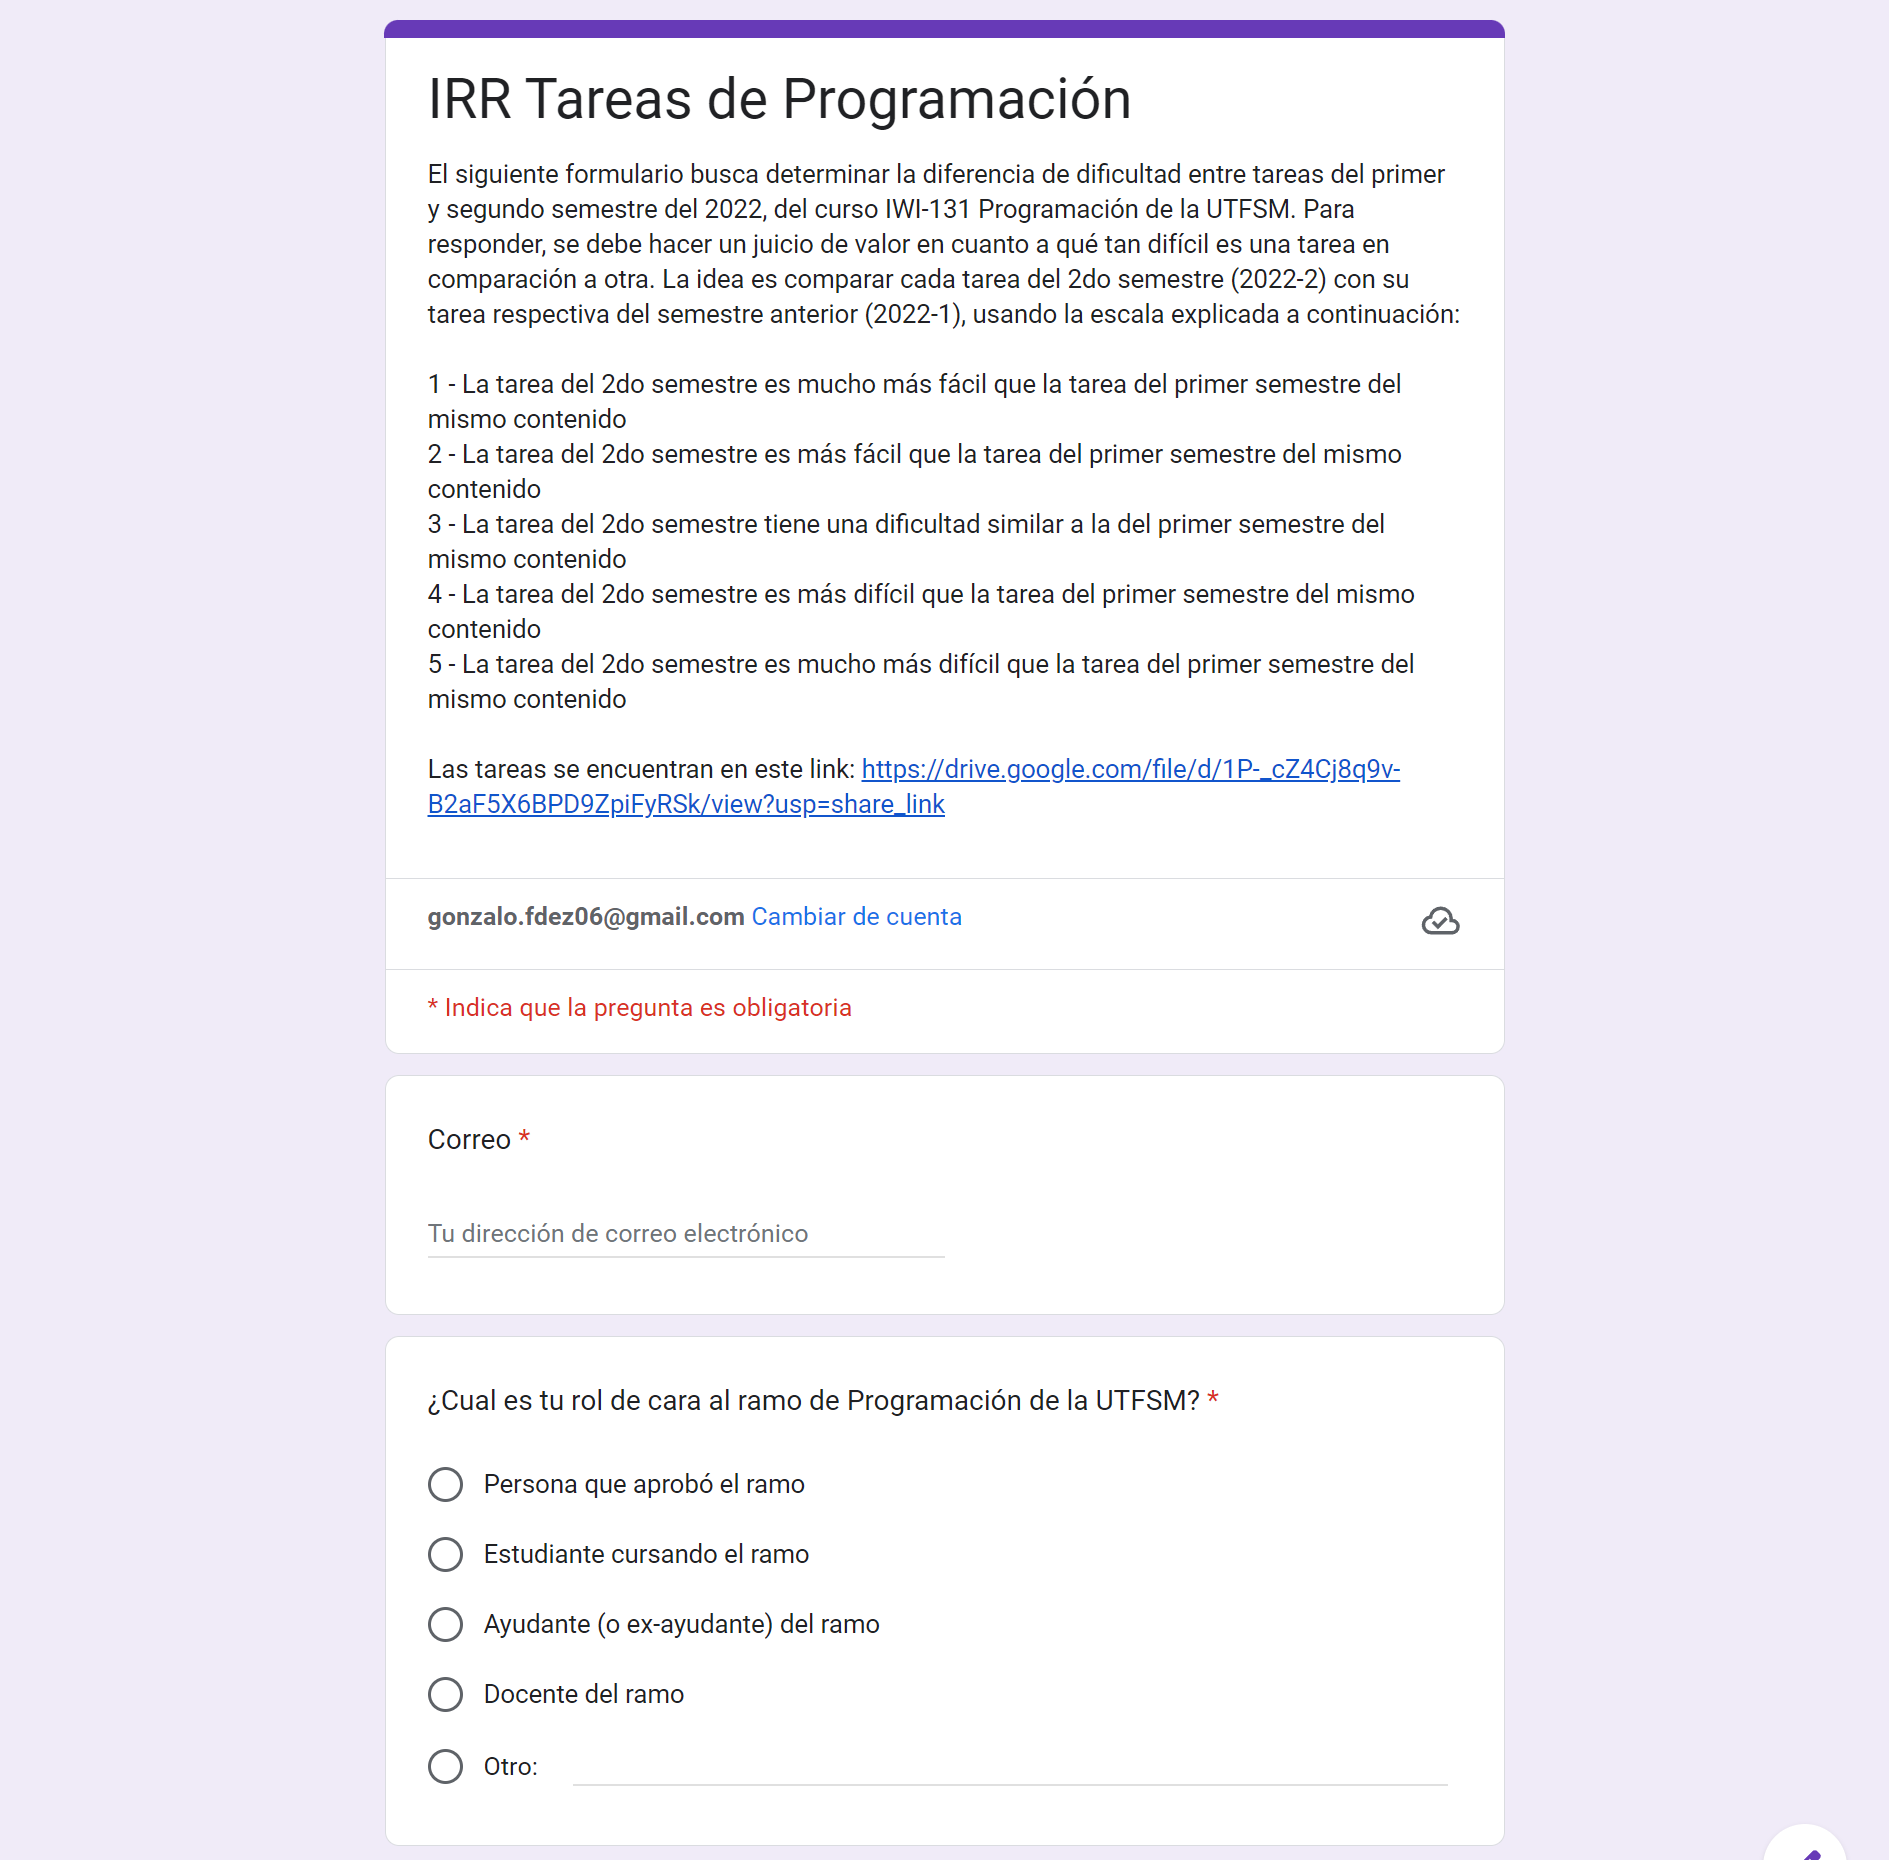
\includegraphics[width=1\textwidth]{figures/formulario1.png}
  \caption{Presentación del formulario para la diferencia de dificultad entre tareas.} Fuente: elaboración propia.
  \label{formulario1}
\end{figure}
\begin{figure}[H]
  \centering
  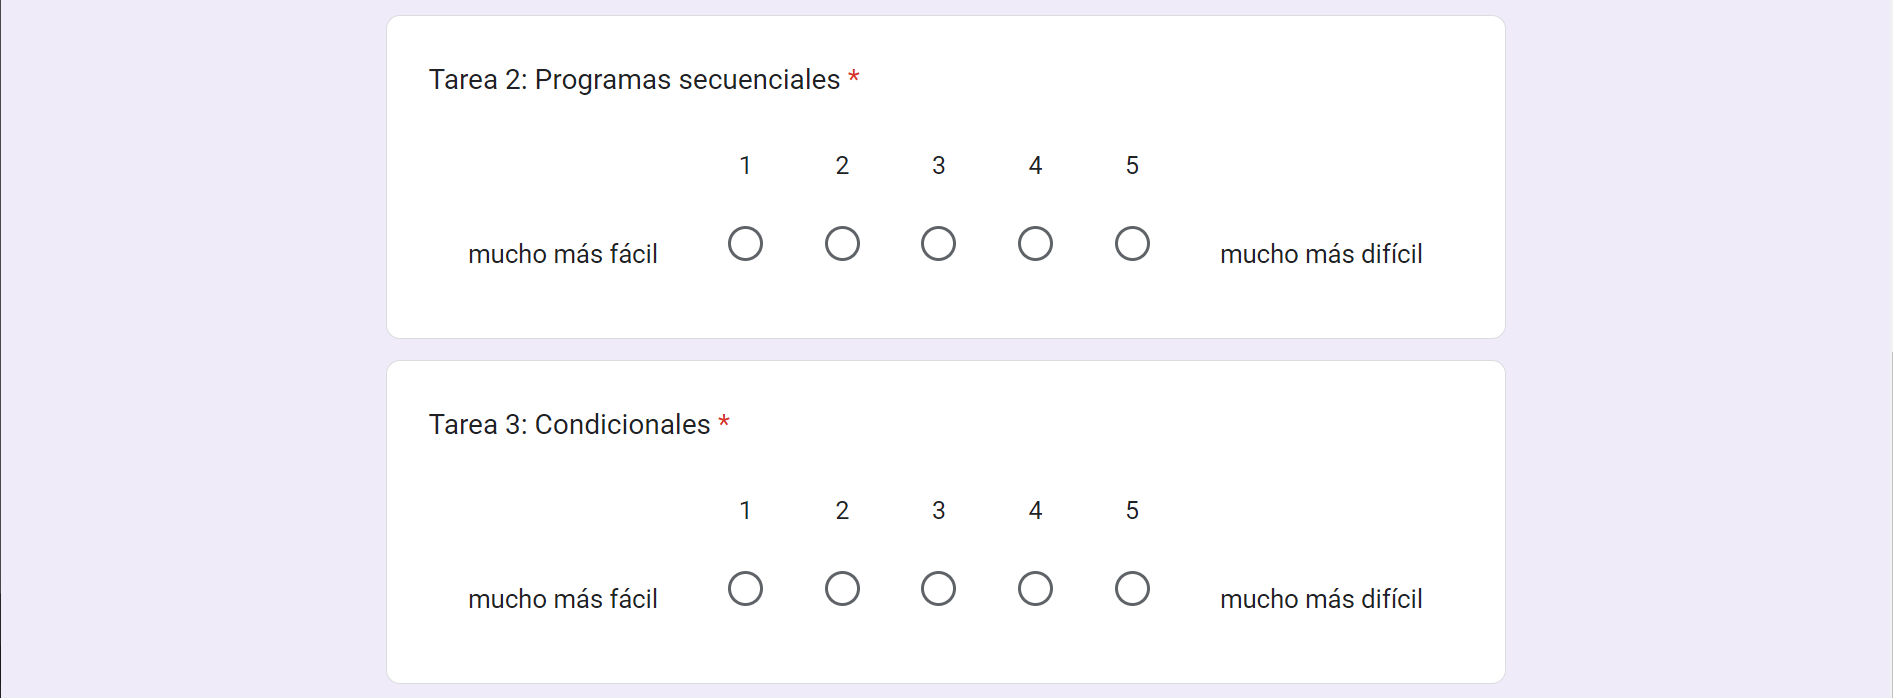
\includegraphics[width=1\textwidth]{figures/formulario2.png}
  \caption{Ejemplo de las preguntas para comparar la dificultad entre 2 tareas de distintos semestres.} Fuente: elaboración propia.
  \label{formulario2}
\end{figure}
La encuesta fue respondida por 2 profesores con años de experiencia en el ramo IWI-131 de la UTFSM como docentes y como coordinadores, y por 3 ayudantes con años de experiencia apoyando el proceso docente del mismo. A continuación se resumen las respuestas:
\begin{table}[H]
  \centering
  \begin{tabular}{|l|r|r|r|r|r|r|r|r|}
    \hline
    \textbf{Rol}      & \multicolumn{1}{l|}{\textbf{Tarea 1}} & \multicolumn{1}{l|}{\textbf{Tarea 2}} & \multicolumn{1}{l|}{\textbf{Tarea 3}} & \multicolumn{1}{l|}{\textbf{Tarea 4}} & \multicolumn{1}{l|}{\textbf{Tarea 5}} & \multicolumn{1}{l|}{\textbf{Tarea 6}} & \multicolumn{1}{l|}{\textbf{Tarea 7}} & \multicolumn{1}{l|}{\textbf{Tarea 8}} \\ \hline
    Ayudante          & 1                                     & 4                                     & 2                                     & 2                                     & 3                                     & 4                                     & 1                                     & 2                                     \\ \hline
    Ayudante          & 1                                     & 3                                     & 2                                     & 3                                     & 3                                     & 3                                     & 2                                     & 3                                     \\ \hline
    Ayudante          & 2                                     & 4                                     & 4                                     & 3                                     & 2                                     & 4                                     & 2                                     & 2                                     \\ \hline
    Docente           & 2                                     & 3                                     & 2                                     & 3                                     & 3                                     & 3                                     & 3                                     & 3                                     \\ \hline
    Docente           & 2                                     & 3                                     & 2                                     & 2                                     & 2                                     & 2                                     & 3                                     & 2                                     \\ \hline
    \rowcolor[HTML]{EFEFEF}
    \textbf{Promedio} & 2                                     & 3                                     & 2                                     & 3                                     & 3                                     & 3                                     & 2                                     & 2                                     \\ \hline
  \end{tabular}
  \caption{Resultado de la encuesta a expertos sobre la diferencia de dificultad entre tareas. }Fuente: Elaboración propia
  \label{tab:encuesta1}
\end{table}
Luego, se calcula la diferencia porcentual entre las métricas de cada una de las tareas utilizando los datos calculados en \ref{sssec:calcMetrics}, obteniendo los siguientes resultados:
\begin{table}[H]
  \centering
  \begin{tabular}{|l|l|r|r|r|r|}
    \hline
    \textbf{Tareas} & \textbf{\begin{tabular}[c]{@{}l@{}}Comparación de\\ dificultad\end{tabular}} & \multicolumn{1}{l|}{\textbf{\begin{tabular}[c]{@{}l@{}}Complejidad \\ ciclomática (dif \%)\end{tabular}}} & \multicolumn{1}{l|}{\textbf{\begin{tabular}[c]{@{}l@{}}Dificultad H. \\ (dif \%)\end{tabular}}} & \multicolumn{1}{l|}{\textbf{\begin{tabular}[c]{@{}l@{}}Esfuerzo \\ (dif \%)\end{tabular}}} & \multicolumn{1}{l|}{\textbf{\begin{tabular}[c]{@{}l@{}}Volumen \\ (dif \%)\end{tabular}}} \\ \hline
    Secuenciales    & 2 - más fácil                                                                & 0,00\%                                                                                                    & -21,46\%                                                                                        & -35,27\%                                                                                   & -17,58\%                                                                                  \\ \hline
    Condicionales   & 3 - similar                                                                  & 26,32\%                                                                                                   & 12,12\%                                                                                         & 3,46\%                                                                                     & -7,72\%                                                                                   \\ \hline
    Ciclos          & 2 - más fácil                                                                & -18,75\%                                                                                                  & -54,06\%                                                                                        & -76,65\%                                                                                   & -49,17\%                                                                                  \\ \hline
    Funciones       & 3 - similar                                                                  & 50,00\%                                                                                                   & 79,59\%                                                                                         & -2,34\%                                                                                    & -45,62\%                                                                                  \\ \hline
    Strings         & 3 - similar                                                                  & 40,00\%                                                                                                   & 3,87\%                                                                                          & -15,12\%                                                                                   & -18,28\%                                                                                  \\ \hline
    Listas          & 3 - similar                                                                  & 54,55\%                                                                                                   & 66,39\%                                                                                         & 515,61\%                                                                                   & 269,97\%                                                                                  \\ \hline
    Archivos        & 2 - más fácil                                                                & -37,50\%                                                                                                  & -2,86\%                                                                                         & -32,65\%                                                                                   & -30,67\%                                                                                  \\ \hline
    Diccionarios    & 2 - más fácil                                                                & 6,25\%                                                                                                    & 43,69\%                                                                                         & -32,61\%                                                                                   & -53,10\%                                                                                  \\ \hline
  \end{tabular}
  \caption{Comparación de dificultad entre tareas, junto con las diferencias porcentuales de cada una de sus métricas} Fuente: elaboración propia
  \label{tab:porcentualDif}
\end{table}

Finalmente, aplicando la heurística de \ref{sssec:calcMetrics}, se obtienen los siguientes intervalos de comparación de dificultad:
\begin{table}[H]
  \centering
  \begin{tabular}{|l|r|r|r|r|}
    \hline
    \textbf{Comparación de Dificultad}     & \multicolumn{1}{l|}{\textbf{Complejidad Ciclomática}} & \multicolumn{1}{l|}{\textbf{Dificultad H.}} & \multicolumn{1}{l|}{\textbf{Esfuerzo}} & \multicolumn{1}{l|}{\textbf{Volumen}} \\ \hline
    \multirow{2}{*}{1 - mucho más fácil}   & \multicolumn{1}{l|}{-inf\%}                           & \multicolumn{1}{l|}{-inf\%}                 & \multicolumn{1}{l|}{-inf\%}            & \multicolumn{1}{l|}{-inf\%}           \\ \cline{2-5}
                                           & -37,51\%                                              & -54,07\%                                    & -76,66\%                               & -53,11\%                              \\ \hline
    \multirow{2}{*}{2 - más fácil}         & -37,50\%                                              & -54,06\%                                    & -76,65\%                               & -53,10\%                              \\ \cline{2-5}
                                           & 6,25\%                                                & 3,87\%                                      & -32,61\%                               & -45,62\%                              \\ \hline
    \multirow{2}{*}{3 - similar}           & 6,26\%                                                & 3,88\%                                      & -32,60\%                               & -45,61\%                              \\ \cline{2-5}
                                           & 26,26\%                                               & 23,88\%                                     & -12,60\%                               & -25,61\%                              \\ \hline
    \multirow{2}{*}{4 - más difícil}       & 26,27\%                                               & 23,89\%                                     & -12,59\%                               & -25,60\%                              \\ \cline{2-5}
                                           & 70,03\%                                               & 81,83\%                                     & 31,46\%                                & -18,11\%                              \\ \hline
    \multirow{2}{*}{5 - mucho más difícil} & 70,04\%                                               & 81,84\%                                     & 31,47\%                                & -18,10\%                              \\ \cline{2-5}
                                           & \multicolumn{1}{l|}{inf\%}                            & \multicolumn{1}{l|}{inf\%}                  & \multicolumn{1}{l|}{inf\%}             & \multicolumn{1}{l|}{inf\%}            \\ \hline
  \end{tabular}
  \caption{Intervalos de dificultad por métrica para cada dificultad comparativa.} Fuente: elaboración propia
  \label{tab:compDif}
\end{table}

\subsubsection{Diferencia de Dificultad entre Tareas del S2022-1 y S2022-2}

Utilizando la tabla \ref{tab:compDif}, se aplican estos intervalos a las diferencias porcentuales de la tabla \ref{tab:porcentualDif}, obteniendo los siguientes resultados por métrica para cada tarea:
\begin{table}[H]
  \centering
  \begin{tabular}{|l|r|r|r|r|r|}
    \hline
    \textbf{Tareas} & \multicolumn{1}{l|}{\textbf{\begin{tabular}[c]{@{}l@{}}Complejidad \\ ciclomática\end{tabular}}} & \multicolumn{1}{l|}{\textbf{Dificultad H.}} & \multicolumn{1}{l|}{\textbf{Esfuerzo}} & \multicolumn{1}{l|}{\textbf{Volumen}} & \multicolumn{1}{l|}{\textbf{Promedio}} \\ \hline
    Secuenciales    & 2                                                                                                & 4                                           & 2                                      & 2                                     & 3                                      \\ \hline
    Condicionales   & 4                                                                                                & 2                                           & 2                                      & 3                                     & 3                                      \\ \hline
    Ciclos          & 2                                                                                                & 2                                           & 2                                      & 2                                     & 2                                      \\ \hline
    Funciones       & 2                                                                                                & 2                                           & 2                                      & 5                                     & 3                                      \\ \hline
    Strings         & 4                                                                                                & 4                                           & 5                                      & 5                                     & 5                                      \\ \hline
    Listas          & 4                                                                                                & 4                                           & 3                                      & 2                                     & 3                                      \\ \hline
    Archivos        & 4                                                                                                & 2                                           & 3                                      & 4                                     & 3                                      \\ \hline
    Diccionarios    & 4                                                                                                & 3                                           & 4                                      & 5                                     & 4                                      \\ \hline
  \end{tabular}
  \caption{Dificultad de las tareas según los intervalos de comparación} Fuente: elaboración propia
  \label{tab:difDifferences}
\end{table}
Al comparar los resultados con las respuestas de la tabla \ref{tab:encuesta1}, se determina que la heurística aplicada para determinar los intervalos de diferencias porcentuales, acertó correctamente a 3 pares de tareas: Ciclos, Funciones y Strings, mientras que para el resto de pareas de tareas, los resultados no estuvieron demasiado alejados de lo determinado por los expertos en la encuesta.

\subsubsection{Actualización de Intervalos de Comparación de Dificultad}

Para cargar la data de los intervalos de dificultad previamente calculados en el framework, se modifica el archivo \texttt{comparisionIntervals.json} según lo que indica la sección \ref{sssec:comparisionIntMod}, resultando:

\begin{figure}[H]
  \centering
  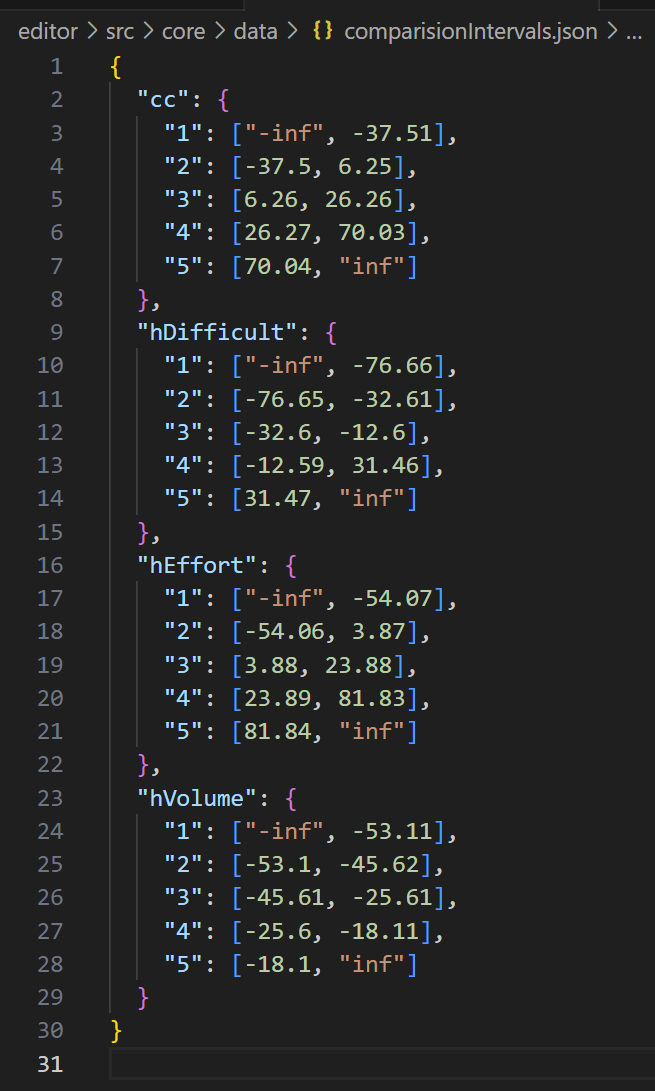
\includegraphics[width=0.4\textwidth]{figures/intervals5.png}
  \caption{Intervalos de comparación de dificultad cargados en el framework.} Fuente: elaboración propia.
  \label{img:intervals5}
\end{figure}

\subsubsection{Actualización de Métricas S2022-1 y S2022-2}

Para cargar la data de las métricas previamente calculados en el framework, se modifican los archivos \texttt{studentAssignments.json} y \texttt{teacherAssignments.json} según lo que indica la sección \ref{sssec:metricsUpdate}, resultando:

\begin{figure}[H]
  \centering
  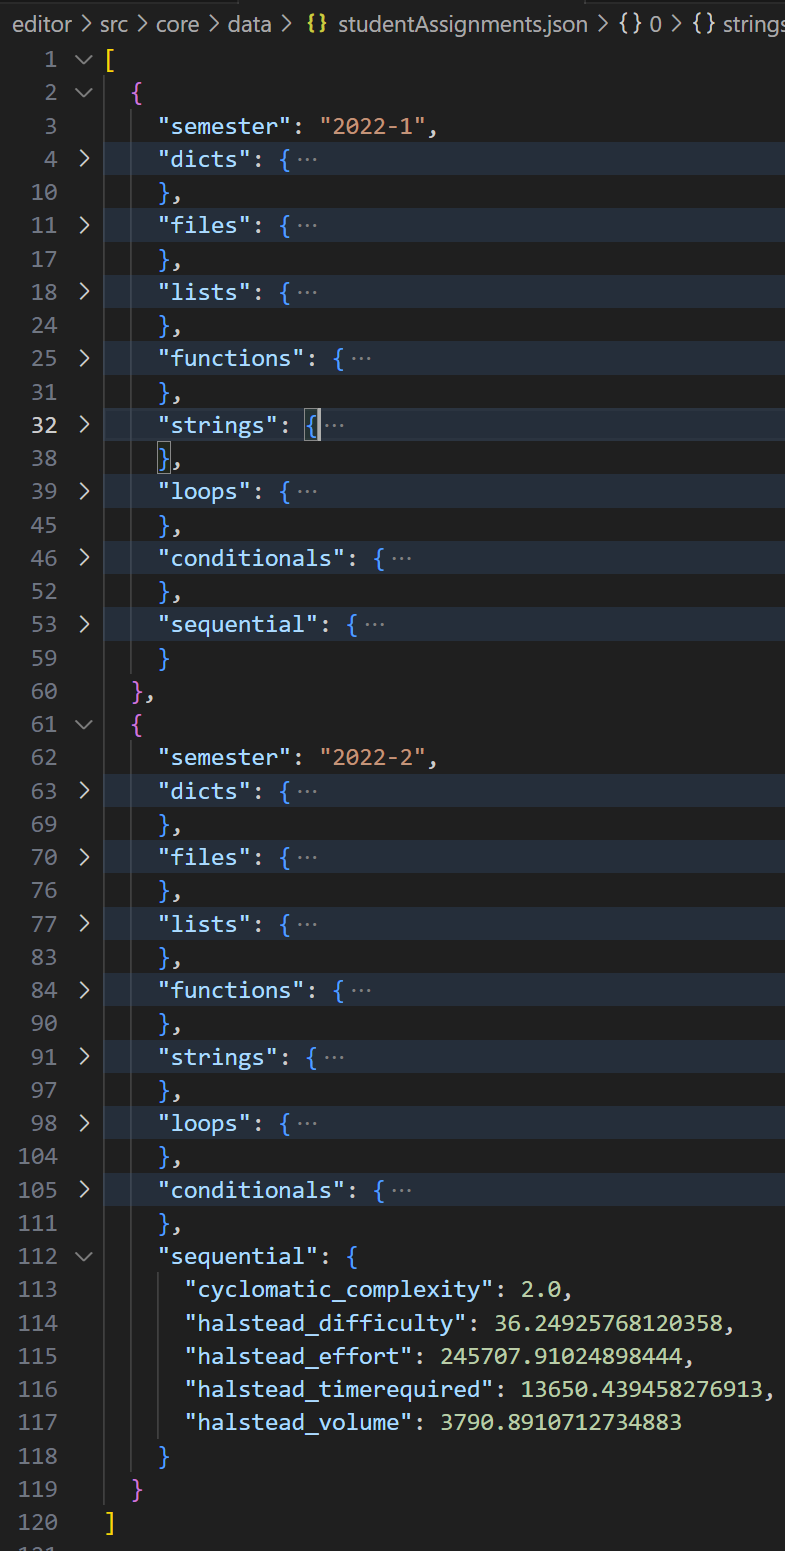
\includegraphics[width=0.4\textwidth]{figures/studentsMetrics1.png}
  \caption{Métricas por semestre de las soluciones de los estudiantes cargados en el framework.} (algunas métricas fueron ocultas para efectos de espacio) Fuente: elaboración propia.
  \label{img:studentsMetrics1}
\end{figure}

\begin{figure}[H]
  \centering
  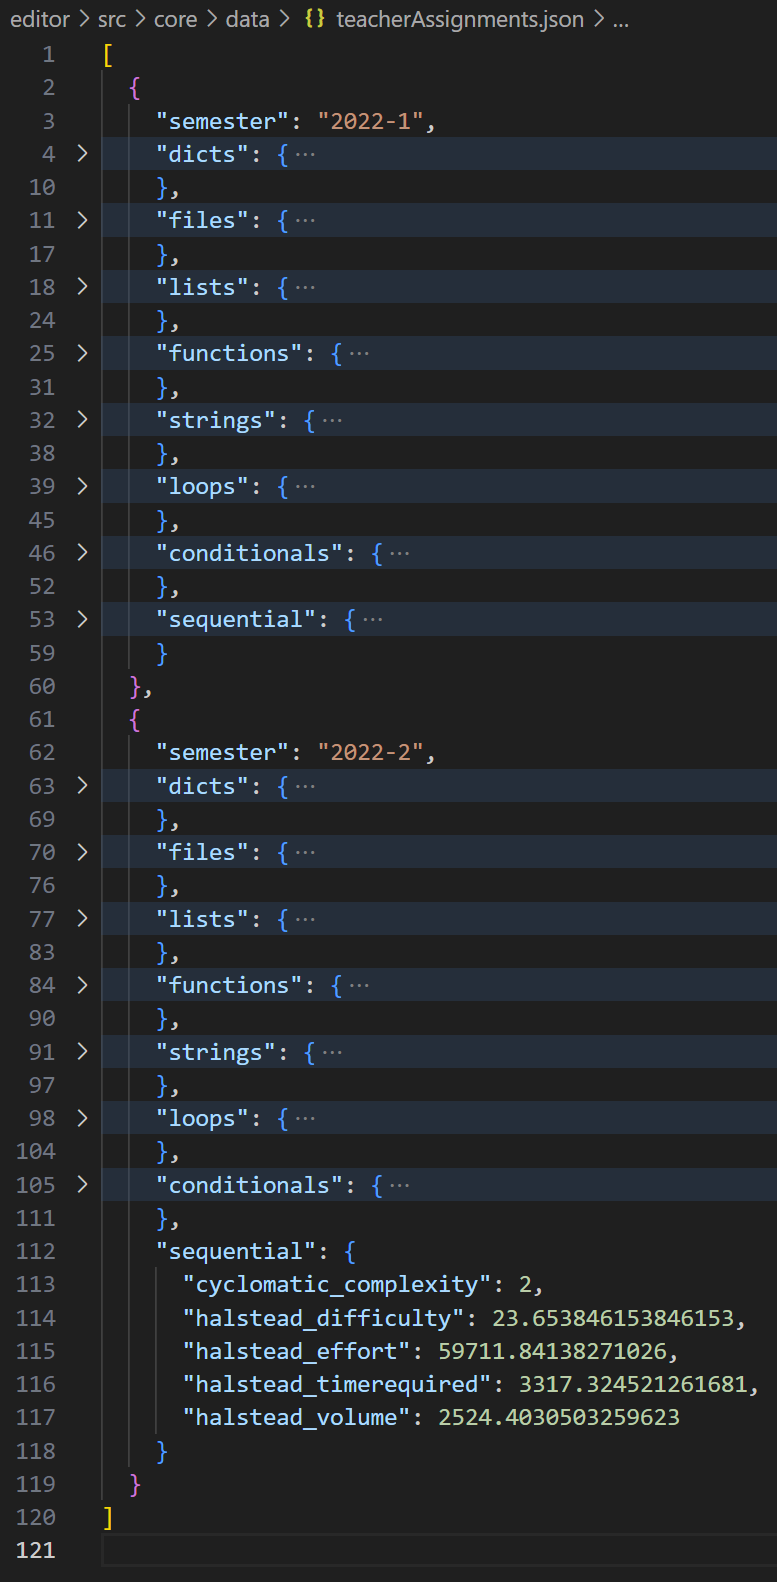
\includegraphics[width=0.4\textwidth]{figures/teacherMetrics1.png}
  \caption{Métricas por semestre de las soluciones de los profesores cargados en el framework.} (algunas métricas fueron ocultas para efectos de espacio) Fuente: elaboración propia.
  \label{img:teacherMetrics1}
\end{figure}

\subsubsection{Redacción de una Tarea con sus Respectivas Métricas}

Siguiendo los pasos de la metodología, se redacta la tarea utilizando el editor de Ishvel:

\begin{figure}[H]
  \centering
  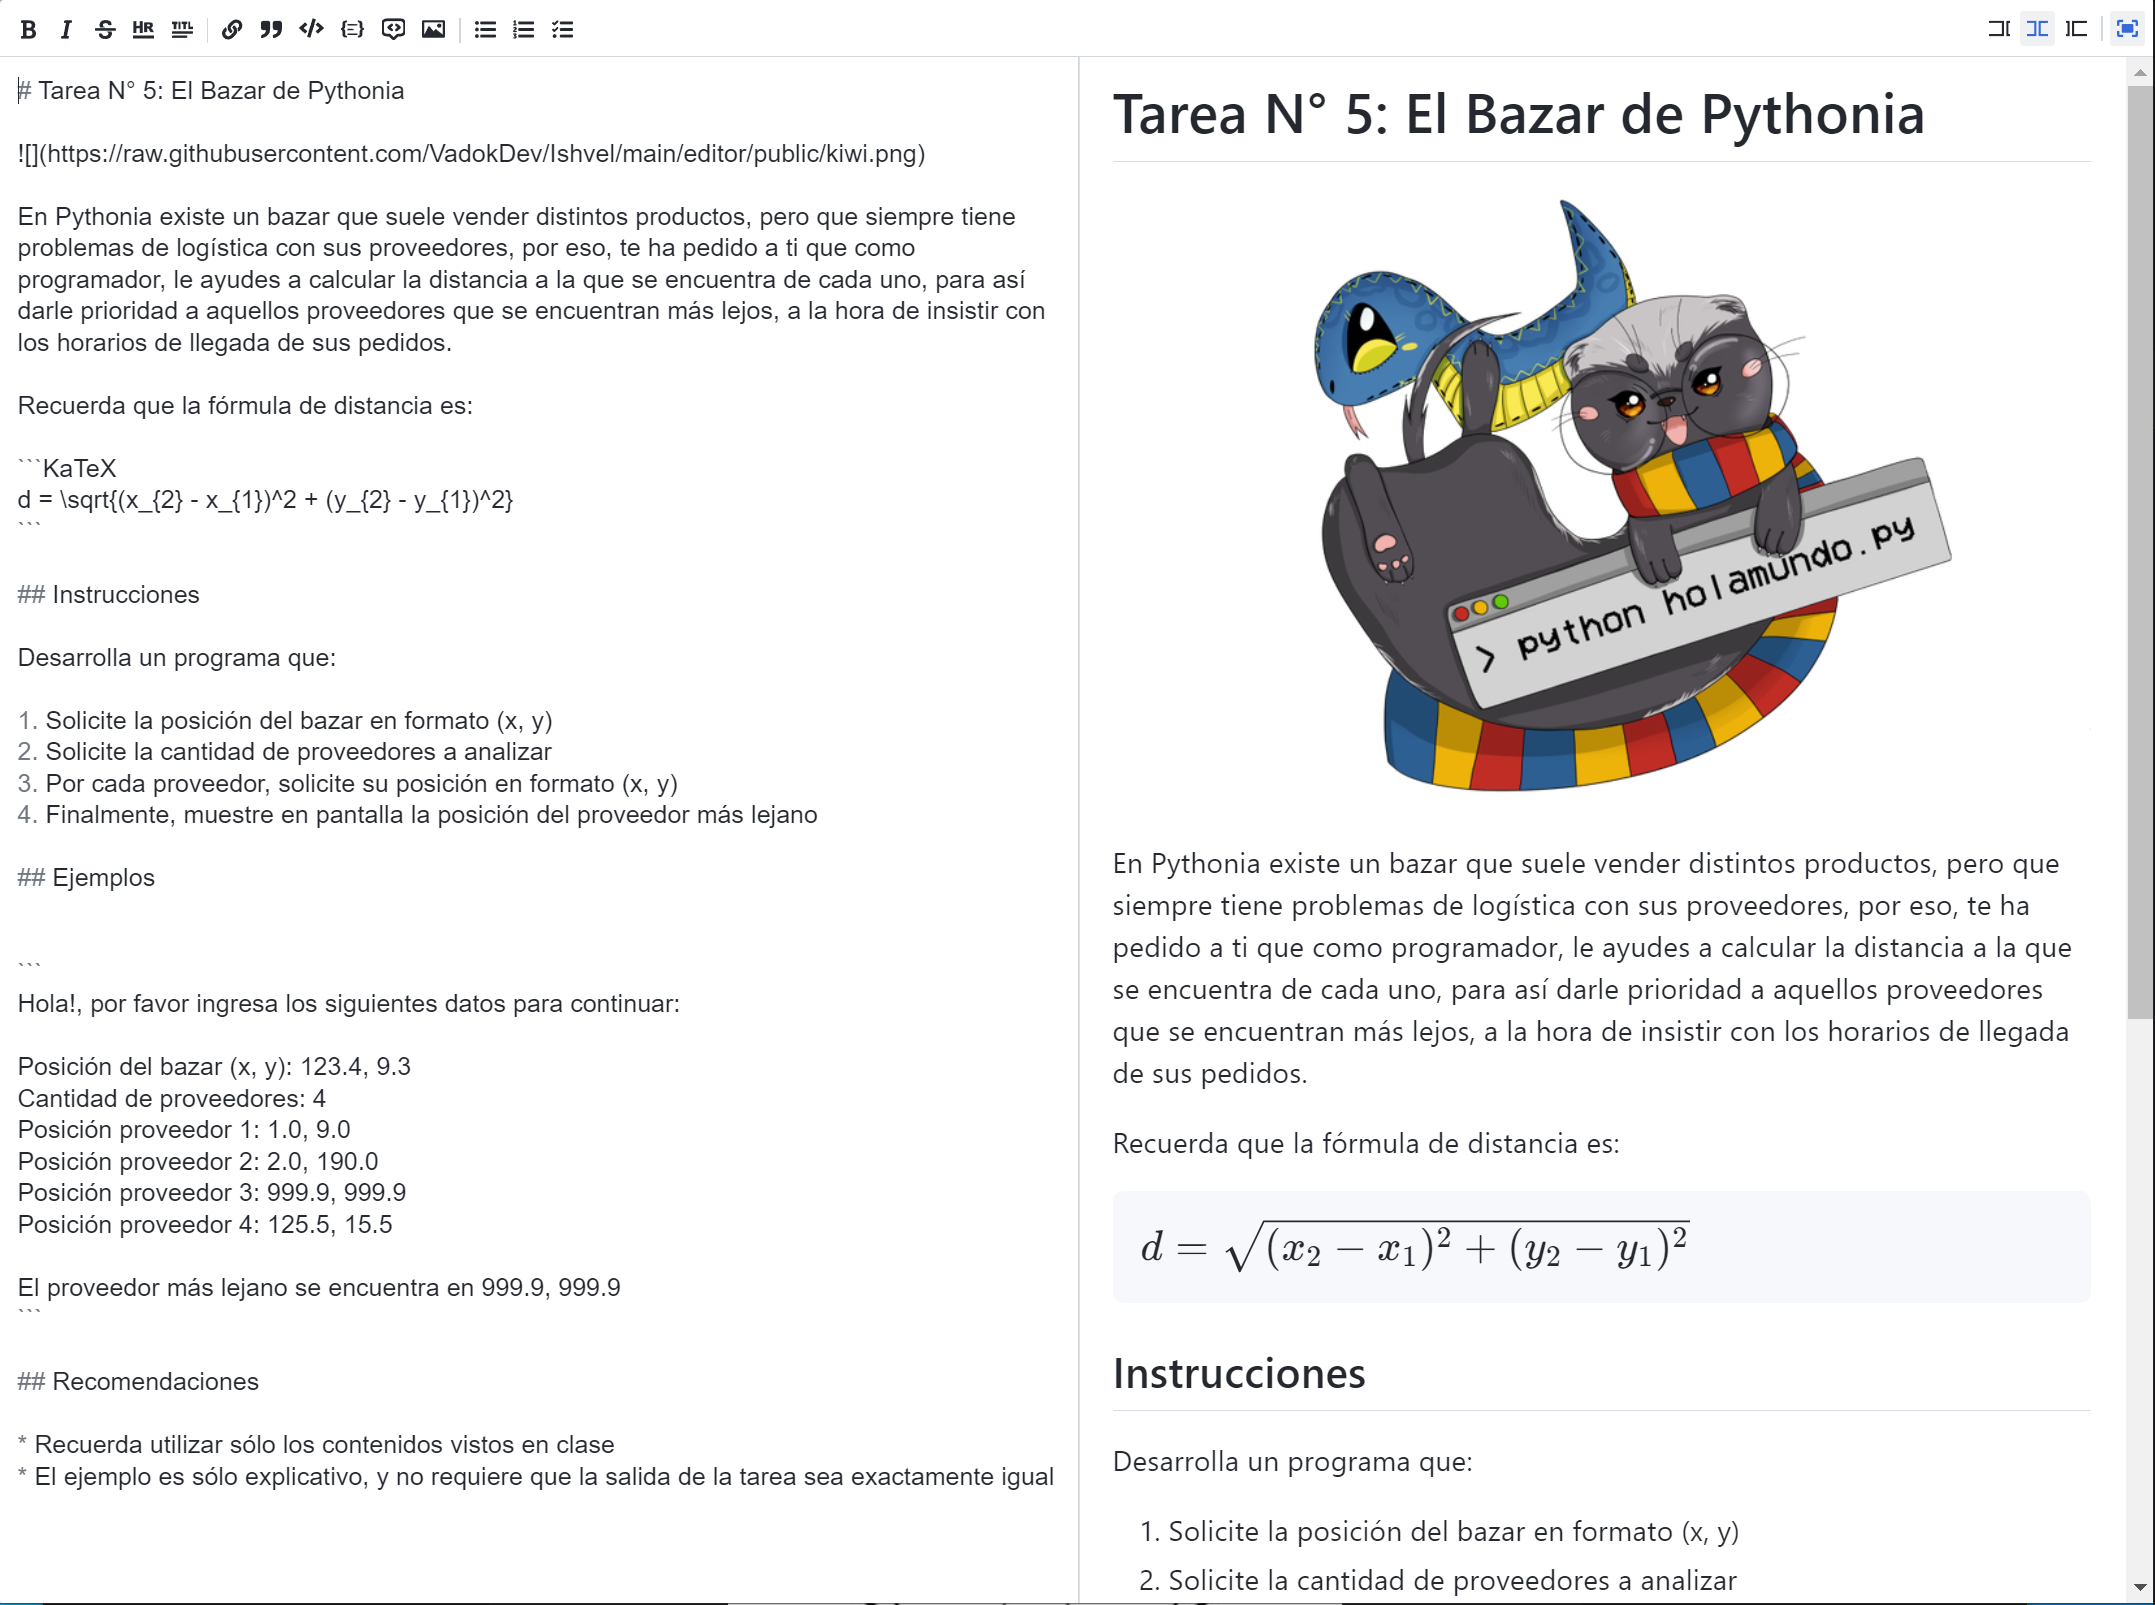
\includegraphics[width=1\textwidth]{figures/ishvel3.png}
  \caption{Tarea elaborada en el editor de Ishvel.} Fuente: elaboración propia.
  \label{img:ishvel8}
\end{figure}

\subsubsection{Comparación de las Tareas de IWI-131 del S2022-1 y S2022-2}


\newpage

\secnumbersection{CONCLUSIONES}

Las Conclusiones son, según algunos especialistas, el aspecto principal de una memoria, ya que reflejan el aprendizaje final del autor del documento. En ellas se tiende a considerar los alcances y limitaciones de la propuesta de solución, establecer de forma simple y directa los resultados, discutir respecto a la validez de los objetivos formulados, identificar las principales contribuciones y aplicaciones del trabajo realizado, así como su impacto o aporte a la organización o a los actores involucrados. Otro aspecto que tiende a incluirse son recomendaciones para quienes se sientan motivados por el tema y deseen profundizarlo, o lineamientos de una futura ampliación del trabajo.

\underline{Todo esto debe sintetizarse en al menos 5 páginas.}

\newpage

\secnumberlesssection{ANEXOS}

\newpage
% Bibliografía estilo APA:
\bibliographystyle{apalike-es}
\bibliography{bibliografia}{}

\end{document}
